\documentclass{beamer}
\usepackage[skins,breakable]{tcolorbox}
\usepackage[english]{babel}
\usetikzlibrary{matrix,backgrounds}
\usepackage{multirow}
\usepackage{hyperref}
\usepackage[notocbib]{apacite}
\usepackage{listings}
\usepackage{color}
\definecolor{deepblue}{rgb}{0,0,0.5}
\definecolor{deepred}{rgb}{0.6,0,0}
\definecolor{deepgreen}{rgb}{0,0.5,0}
\usepackage{stackengine}
\setbeamercovered{invisible}
\usepackage{multicol}
\usepackage{adjustbox}
\usepackage{soul}
\usepackage{pgfplots}
\usepackage[outputdir=build]{minted}
\usepackage{listings}
\usepackage{subfig}
\usepackage{amssymb}% http://ctan.org/pkg/amssymb
\usepackage{pifont}% http://ctan.org/pkg/pifont
\usepackage{graphicx}% http://ctan.org/pkg/graphicx
\usepackage{booktabs}% http://ctan.org/pkg/booktabs
\usepackage{tikz}
\usetikzlibrary{shapes.geometric, arrows, chains, calc,positioning,fit,decorations.pathreplacing}
\usepackage[framemethod=tikz]{mdframed}
\definecolor{light-gray}{gray}{0.95}

% Default fixed font does not support bold face
\DeclareFixedFont{\ttb}{T1}{txtt}{bx}{n}{12} % for bold
\DeclareFixedFont{\ttm}{T1}{txtt}{m}{n}{12}  % for normal

% Custom colors
\definecolor{deepblue}{rgb}{0,0,0.5}
\definecolor{deepred}{rgb}{0.6,0,0}
\definecolor{deepgreen}{rgb}{0,0.5,0}

\usepackage{listings}

% Python style for highlighting
\newcommand\pythonstyle{\lstset{
language=Python,
mathescape=true,
basicstyle=\ttm,
otherkeywords={self},             % Add keywords here
keywordstyle=\ttb\color{deepblue},
emph={MyClass,__init__},          % Custom highlighting
emphstyle=\ttb\color{deepred},    % Custom highlighting style
stringstyle=\color{deepgreen},
frame=tb,                         % Any extra options here
showstringspaces=false            %
}}


% Python environment
\lstnewenvironment{python}[1][]
{
\pythonstyle
\lstset{#1}
}
{}

% Python for external files
\newcommand\pythonexternal[2][]{{
\pythonstyle
\lstinputlisting[#1]{#2}}}

% Python for inline
\newcommand\pythoninline[1]{{\pythonstyle\lstinline!#1!}}

\lstset{
  breaklines=true,
  postbreak=\mbox{\textcolor{red}{$\hookrightarrow$}\space},
  mathescape = true,
  basicstyle=\ttm,
  keywordstyle=\ttb\color{deepblue},
  emph={MyClass,__init__},          % Custom highlighting
  emphstyle=\ttb\color{deepred},    % Custom highlighting style
  stringstyle=\color{deepgreen},
  frame=tb,                         % Any extra options here
  showstringspaces=false,            %
  aboveskip=20pt,
  belowskip=20pt
}
\graphicspath{ {./img/}}
\usepackage[utf8]{inputenc}
\usetheme{PaloAlto}
\setbeamerfont{section in sidebar}{size=\fontsize{2}{4}\selectfont}
\setbeamerfont{subsection in sidebar}{size=\fontsize{2}{3}\selectfont}
\setbeamerfont{subsubsection in sidebar}{size=\fontsize{2}{2}\selectfont}

\setbeamerfont{section in toc}{size=\footnotesize}
\setbeamerfont{subsection in toc}{size=\scriptsize}
\setbeamerfont{subsubsection in toc}{size=\tiny}

\hypersetup{
    urlcolor=cyan           % color of external links
}


\title{HOW-R-U?}
\date{17th July 2020}
\subtitle{Suite of e-coaches aimed to analyse human behaviour}

\author{Carlos Sánchez Páez\\Oresti Baños Legrán}

\makeatletter
  \setbeamertemplate{sidebar \beamer@sidebarside}%{sidebar theme}
  {
    \beamer@tempdim=\beamer@sidebarwidth%
    \advance\beamer@tempdim by -6pt%
    \insertverticalnavigation{\beamer@sidebarwidth}%
    \vfill
    \ifx\beamer@sidebarside\beamer@lefttext%
    \else%
      \usebeamercolor{normal text}%
      \llap{\usebeamertemplate***{navigation symbols}\hskip0.1cm}%
      \vskip2pt%
    \fi%
}%
\addtobeamertemplate{navigation symbols}{}{%
    \usebeamerfont{footline}%
    \usebeamercolor[fg]{footline}%
    \hspace{1em}%
    \insertframenumber/\inserttotalframenumber
}
\makeatother
\newcommand{\greentick}{\textcolor{green}{\ding{52}}}
\newcommand{\redcross}{\textcolor{red}{\ding{55}}}

\subject{HOW-R-U?: Suite of e-coaches aimed to analyse human behaviour}

% Let's get started
\begin{document}
\AtBeginSection[]
  {
     \begin{frame}<beamer>
     \frametitle{Index}
     \tableofcontents[currentsection]
     \end{frame}
  }
\AtBeginSubsection[]
{
  \begin{frame}<beamer>{Index}
    \tableofcontents[currentsection,currentsubsection]
  \end{frame}
}
\AtBeginSubsubsection[]
{
  \begin{frame}<beamer>{Index}
    \tableofcontents[currentsection,currentsubsection]
  \end{frame}
}
\centering
\begin{frame}
 \titlepage
\end{frame}

\begin{frame}{Índice}
 \tableofcontents
 % You might wish to add the option [pausesections]
\end{frame}

\section{Introduction}
\subsection{Proposal}
\begin{frame}[fragile]{Proposal}
  \begin{itemize}[<+->]
    \item \emph{E-coaches} suite as chatbots.
    \item Doctors can assign questions to patients.
    \item Data analysis.
    \item Psychologist bot.
  \end{itemize}
\end{frame}
\subsection{Context and motivation}
\begin{frame}[fragile]{Context}
  \begin{itemize}[<+->]
    \item Mental disorders are very common in our society.
    \item Doctors have high workloads.
    \item Mental diseases are taboo.
    \item No continuous traceability of patient's health status.
  \end{itemize}
\end{frame}

\begin{frame}[fragile]{Context}
\begin{figure}[H]
  \centering
  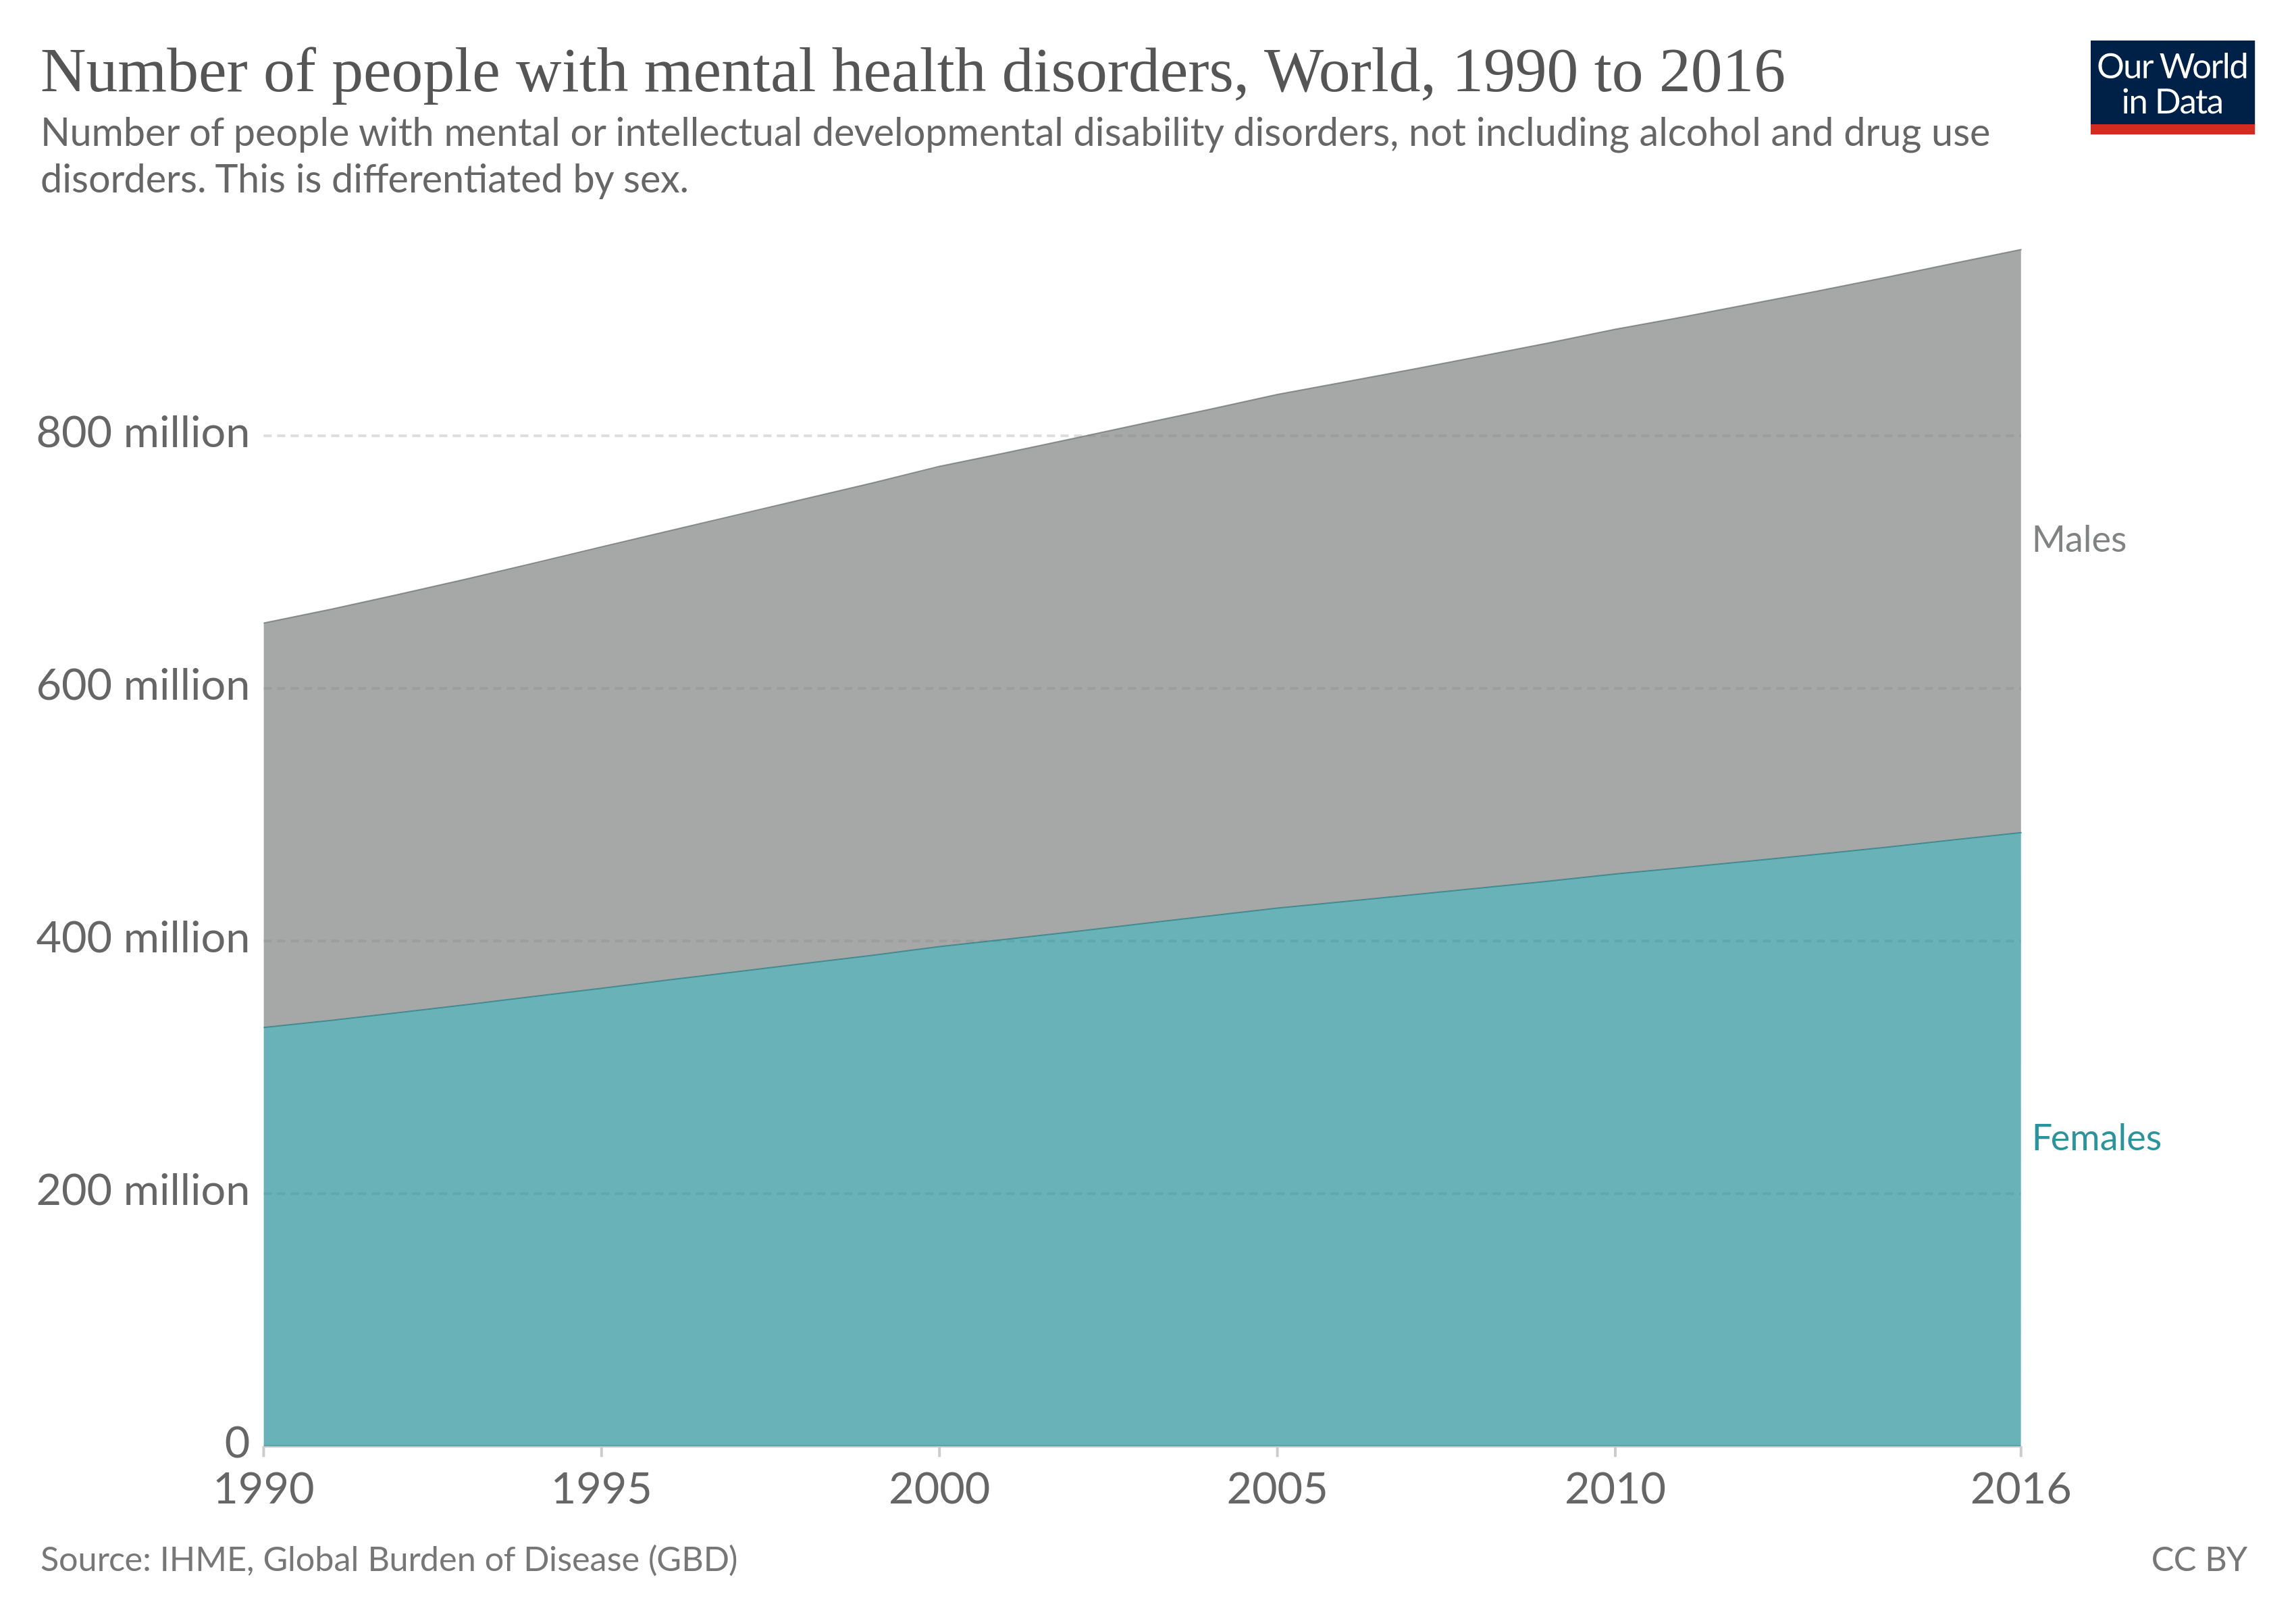
\includegraphics[width=0.8\textwidth]{number_mental_health.png}
  \caption{Number of people with mental health disorders}{Reprinted from \cite{owidmentalhealth}.}
\end{figure}
\end{frame}
%%%%%%%%%%%%%%%%%%%%%%%%%%%%%%%%%%%%%%%%%%%%%%%%%%%%%%%%
\begin{frame}[fragile]{Motivation}
  \begin{itemize}[<+->]
    \item Technology is becoming increasingly integrated into our lives.
    \item Smartphones are used in a daily basis.
    \item Chatbots are becoming growingly becoming popular.
    \item In Spain there are 2 psychologist per 100.000 citizens \cite{elmundo}.
  \end{itemize}
\end{frame}
%%%%%%%%%%%%%%%%%%%%%%%%%%%%%%%%%%%%%%%
\subsection{Objectives}
\begin{frame}[fragile]{Objectives}
  \begin{itemize}[<+->]
    \item \textbf{Main goal}:
    \begin{itemize}[<+->]
      \item \emph{Conversational-agent-as-a-sensor} that asks questions to patients.
      \item Questions will be defined by specialists.
    \end{itemize}
    \item \textbf{Secondary goals}.
      \begin{itemize}[<+->]
        \item Graphical web interface for doctors.
        \item Flexible and scalable architecture to add functionality to the system.
        \item Architecture based on containers to host the different system modules.
        \item Implement a system that covers the previous goals.
        \item Test a beta version of the system to retrieve target audience’s feelings about it.
      \end{itemize}
  \end{itemize}
\end{frame}
\section{State of the art}

\subsection{Publications related to chatbots}
\begin{frame}[fragile]{Number of publications related to chatbots}
  \begin{figure}
    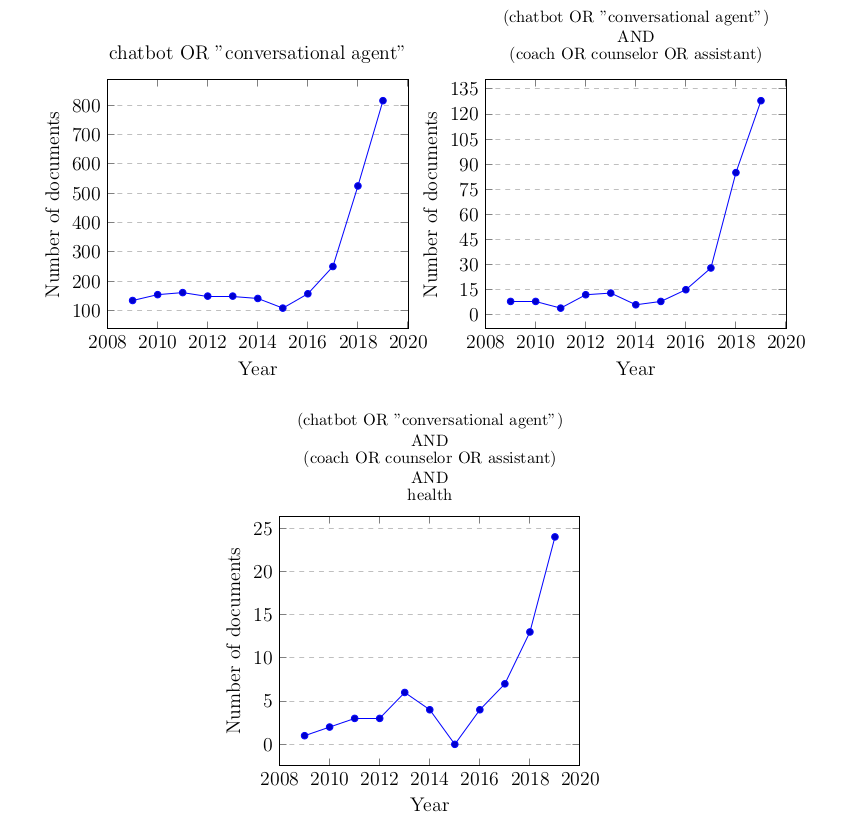
\includegraphics[width=0.68\textwidth]{publications.png}
    \caption{Search results of different queries performed in \textit{scopus.com}.}
  \end{figure}
\end{frame}
\subsection{Health application domains}
\begin{frame}[fragile]{Health application domains}
  \begin{itemize}[<+->]
    \item Areas of application.
    \begin{itemize}[<+->]
      \item Dermathology
      \item Nutrition
      \item Psychology
      \item etc.
    \end{itemize}
    \item Target group.
    \begin{itemize}[<+->]
      \item Students
      \item Doctors
      \item Patients
    \end{itemize}
  \end{itemize}
\end{frame}


\subsection{Conversational agent types and communication formats}

\begin{frame}[fragile]{Conversational agent types}
  \begin{itemize}[<+->]
    \item Coaches: help users to get what they want.
    \item Counselors: help users to identify and solve problems.
  \end{itemize}
\end{frame}
%%%%%%%%%%%%%%%%%%%%%%%%%%%%%%%%%%%%%%%%%%%%%%%%%%%%%%%%%%%%
\begin{frame}[fragile]{Communication formats}
  \begin{itemize}[<+->]
    \item Text
    \item Voice
    \item Multimodal
  \end{itemize}
\end{frame}
\subsection{Technology}

\begin{frame}[fragile]{Technology}
  \begin{table}[h!]
    \centering
    \begin{tabular}{|c|c|c|c|}
      \hline
      \textbf{Platform} & \addstackgap{\textbf{\shortstack{Daily \\ active users\\(billions)}}} & \textbf{\shortstack{Free API \\for chatbots}}  \\
      \hline
      \cite{FacebookMessenger} & 1.66 &  \greentick  \\
      \hline
      \cite{Whatsapp} & 1.5 & \redcross \\
      \hline
      \cite{WeChat} & 1.083 & \greentick  \\
      \hline
      \cite{Telegram} & 0.2 & \greentick \\
      \hline
      \cite{Kik} & 0.015 & \greentick \\
      \hline
      \cite{Discord} & 0.014 & \greentick \\
      \hline
      \cite{Slack} & 0.012 &  \greentick \\
      \hline
      \cite{Viber} & 0.008 &  \greentick \\
      \hline
      \cite{Line} & 0.00723 & \greentick  \\
      \hline
    \end{tabular}
    \caption{Comparison between different chat applications (2019).}
  \end{table}
\end{frame}

\begin{frame}[fragile]{Technology}
  \begin{itemize}[<+->]
    \item Facebook likes can be helpful to predict people's sensitive properties \cite{Kosinski5802}.
    \item Whatsapp's end-to-end encryption methods are not secure enough \cite{Rastogi17}.
    \item Telegram provides more privacy protection \cite{Sutikno16}.
  \end{itemize}
\end{frame}

\section{Methodology}
\subsection{Requirements}

\begin{frame}[fragile]{Requirements}
  \begin{itemize}[<+->]
    \item \emph{Must have} requirements.
      \begin{itemize}[<+->]
        \item Ask questions to the patients.
        \item Custom keyboard.
        \item User's enrollment and deletion.
        \item File with patients' answers.
        \item Modularity.
      \end{itemize}
    \item \emph{Should have} requirements.
      \begin{itemize}[<+->]
        \item CC BY-NC-SA 4.0 \cite{CC} license.
        \item Questions and answers should be modifiable.
        \item Public questions.
        \item Configurable schedule.
        \item Interactive charts.
       \end{itemize}
  \end{itemize}
\end{frame}
%%%%%%%%%%%%%%%%%%%%%%%%%%%%%%%%%%%%%%%%%%%%%%%%%
\begin{frame}[fragile]{Requirements}
  \begin{itemize}[<+->]
    \item \emph{Could have} requirements.
          \begin{itemize}[<+->]
            \item Numeric order of questions.
            \item Custom questions frequency.
            \item Other languages.
            \item Password change.
            \item Two factor authentication.
            \item Groups.
            \item Delete data from users.
            \item View and modify profile data.
            \item Assign questions to all patients.
            \item Timezones support.
          \end{itemize}
        \item \emph{Won't have} requirements.
          \begin{itemize}[<+->]
            \item Cross-platform.
            \item Share the retrieved data with third parties.
          \end{itemize}
  \end{itemize}
\end{frame}

\subsection{Architecture}
\begin{frame}[fragile]{Architecture}
\begin{figure}[H]
    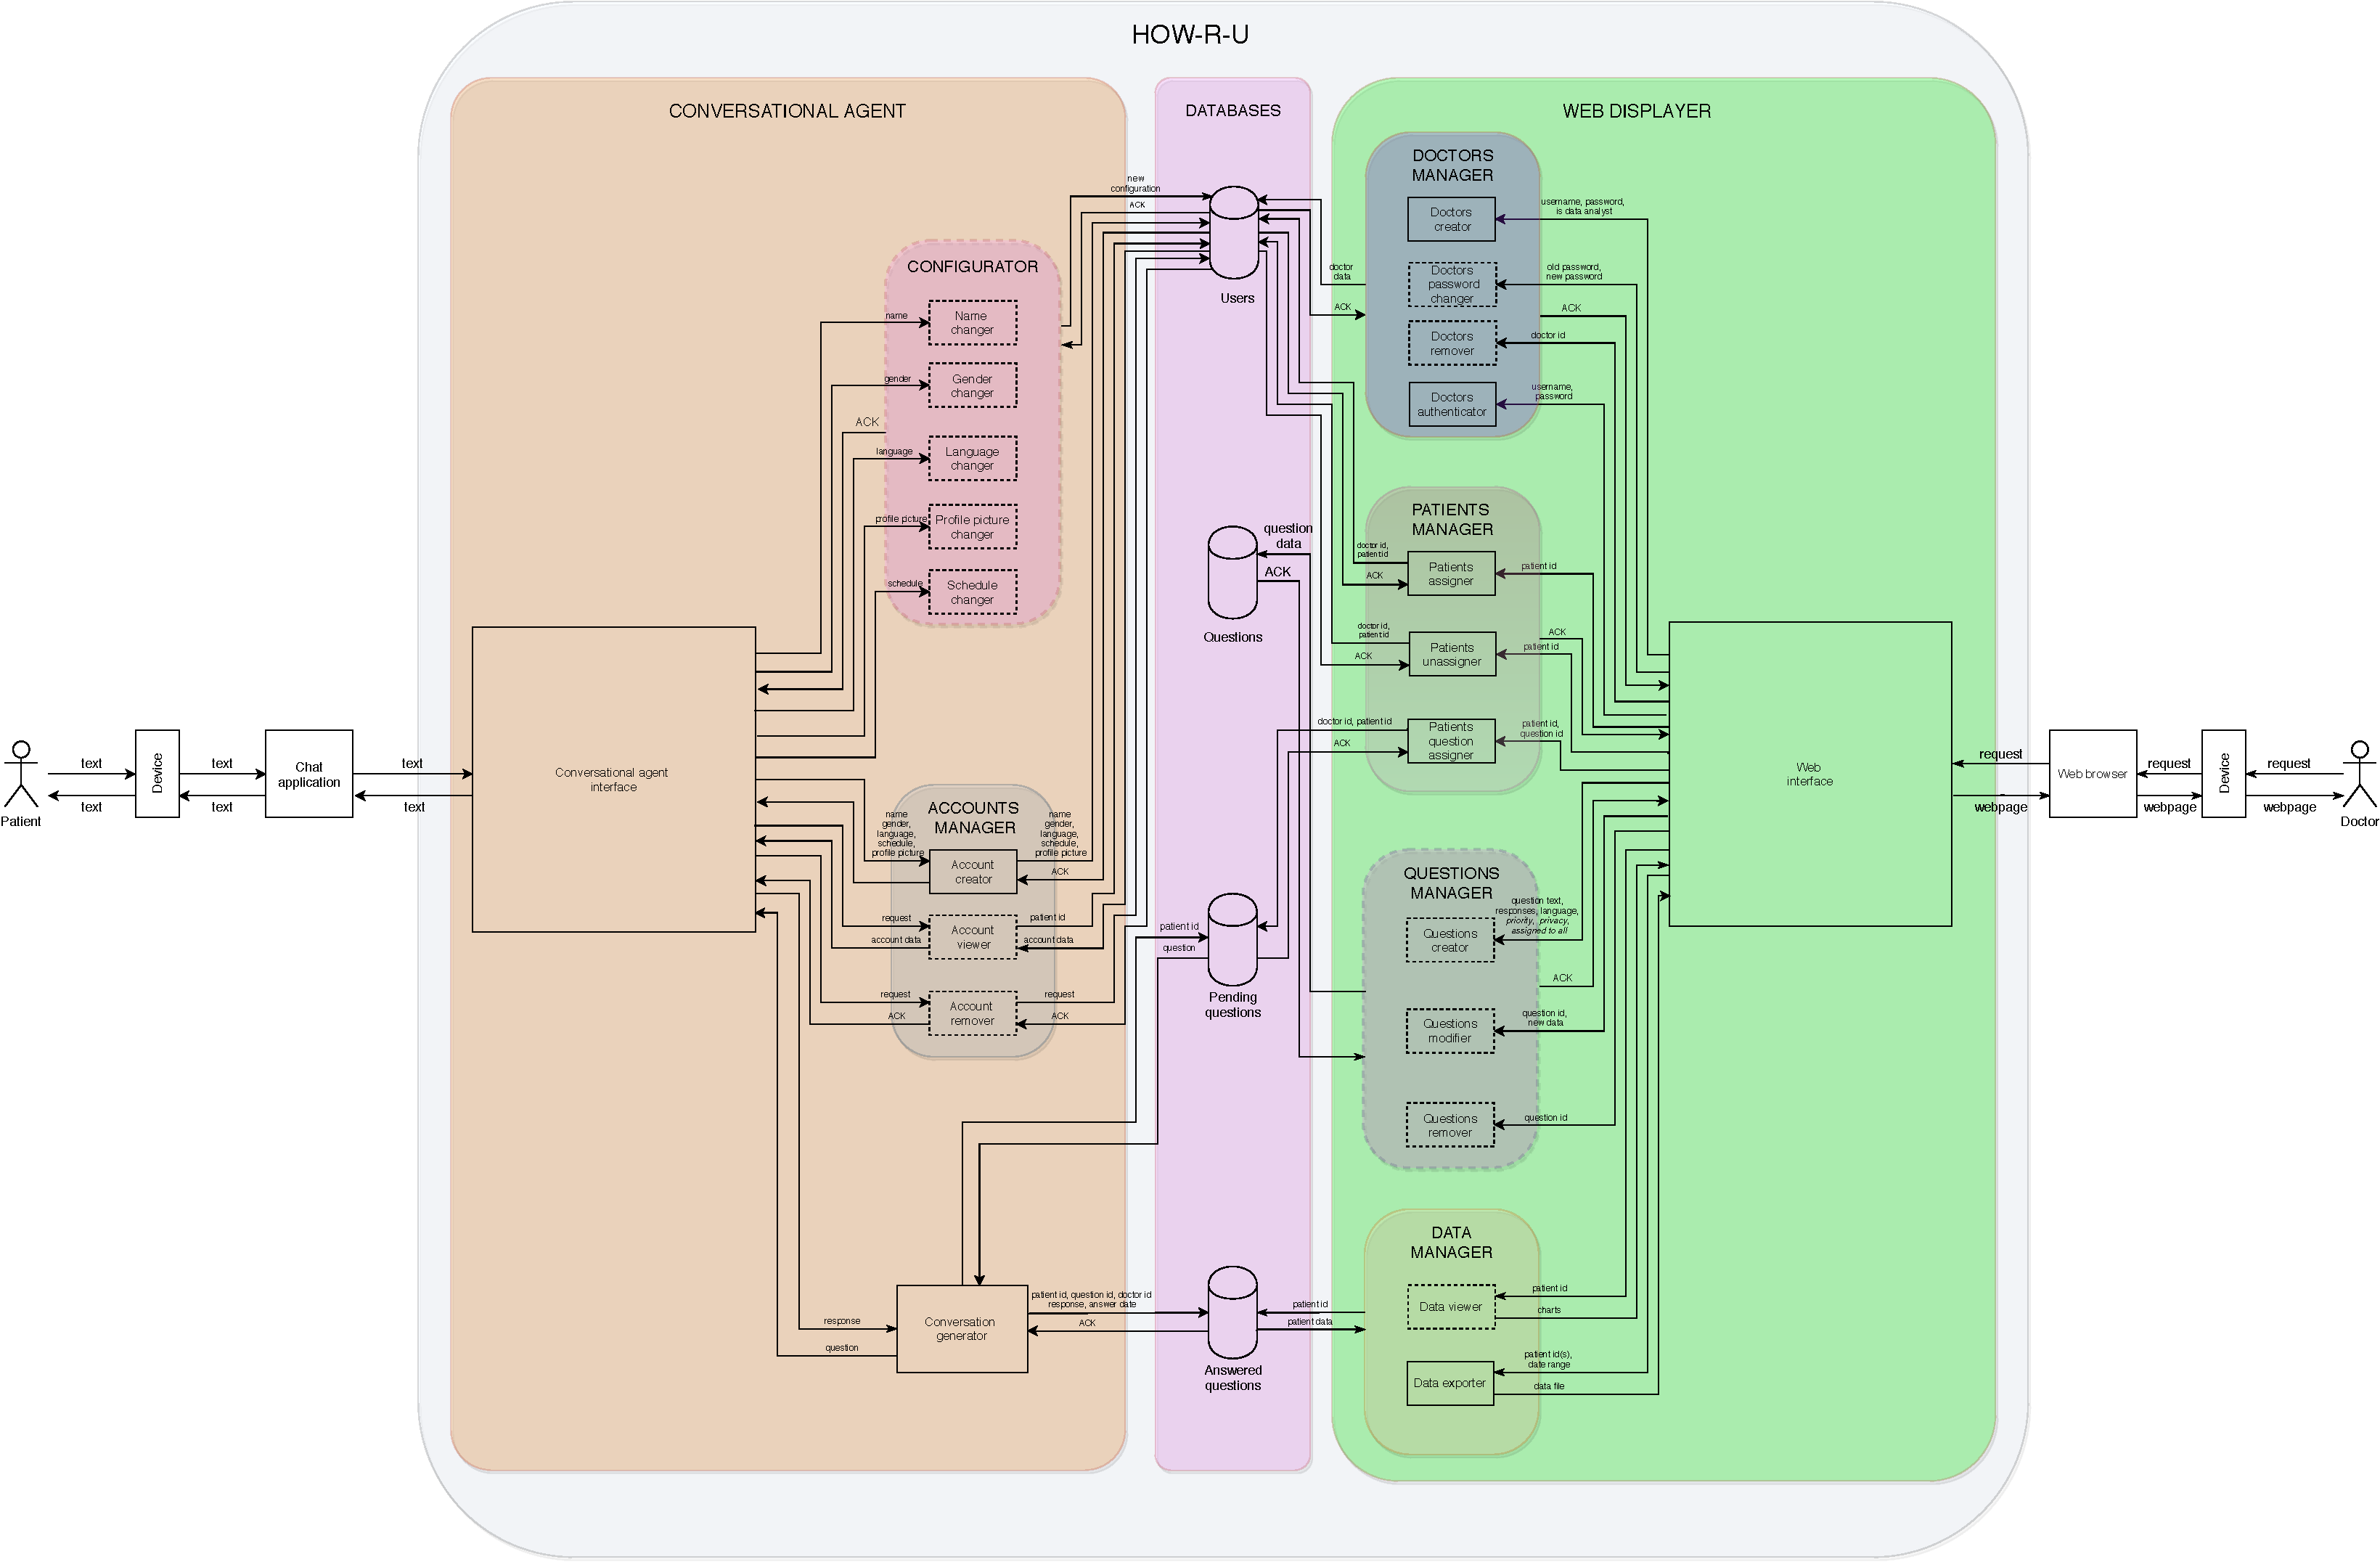
\includegraphics[width=0.9\textwidth]{architecture.pdf}
    \caption{System architecture. Created using \emph{diagrams.net} \protect\cite{drawio}.}
\end{figure}
\end{frame}

\begin{frame}[fragile]{Architecture}
\begin{figure}[H]
    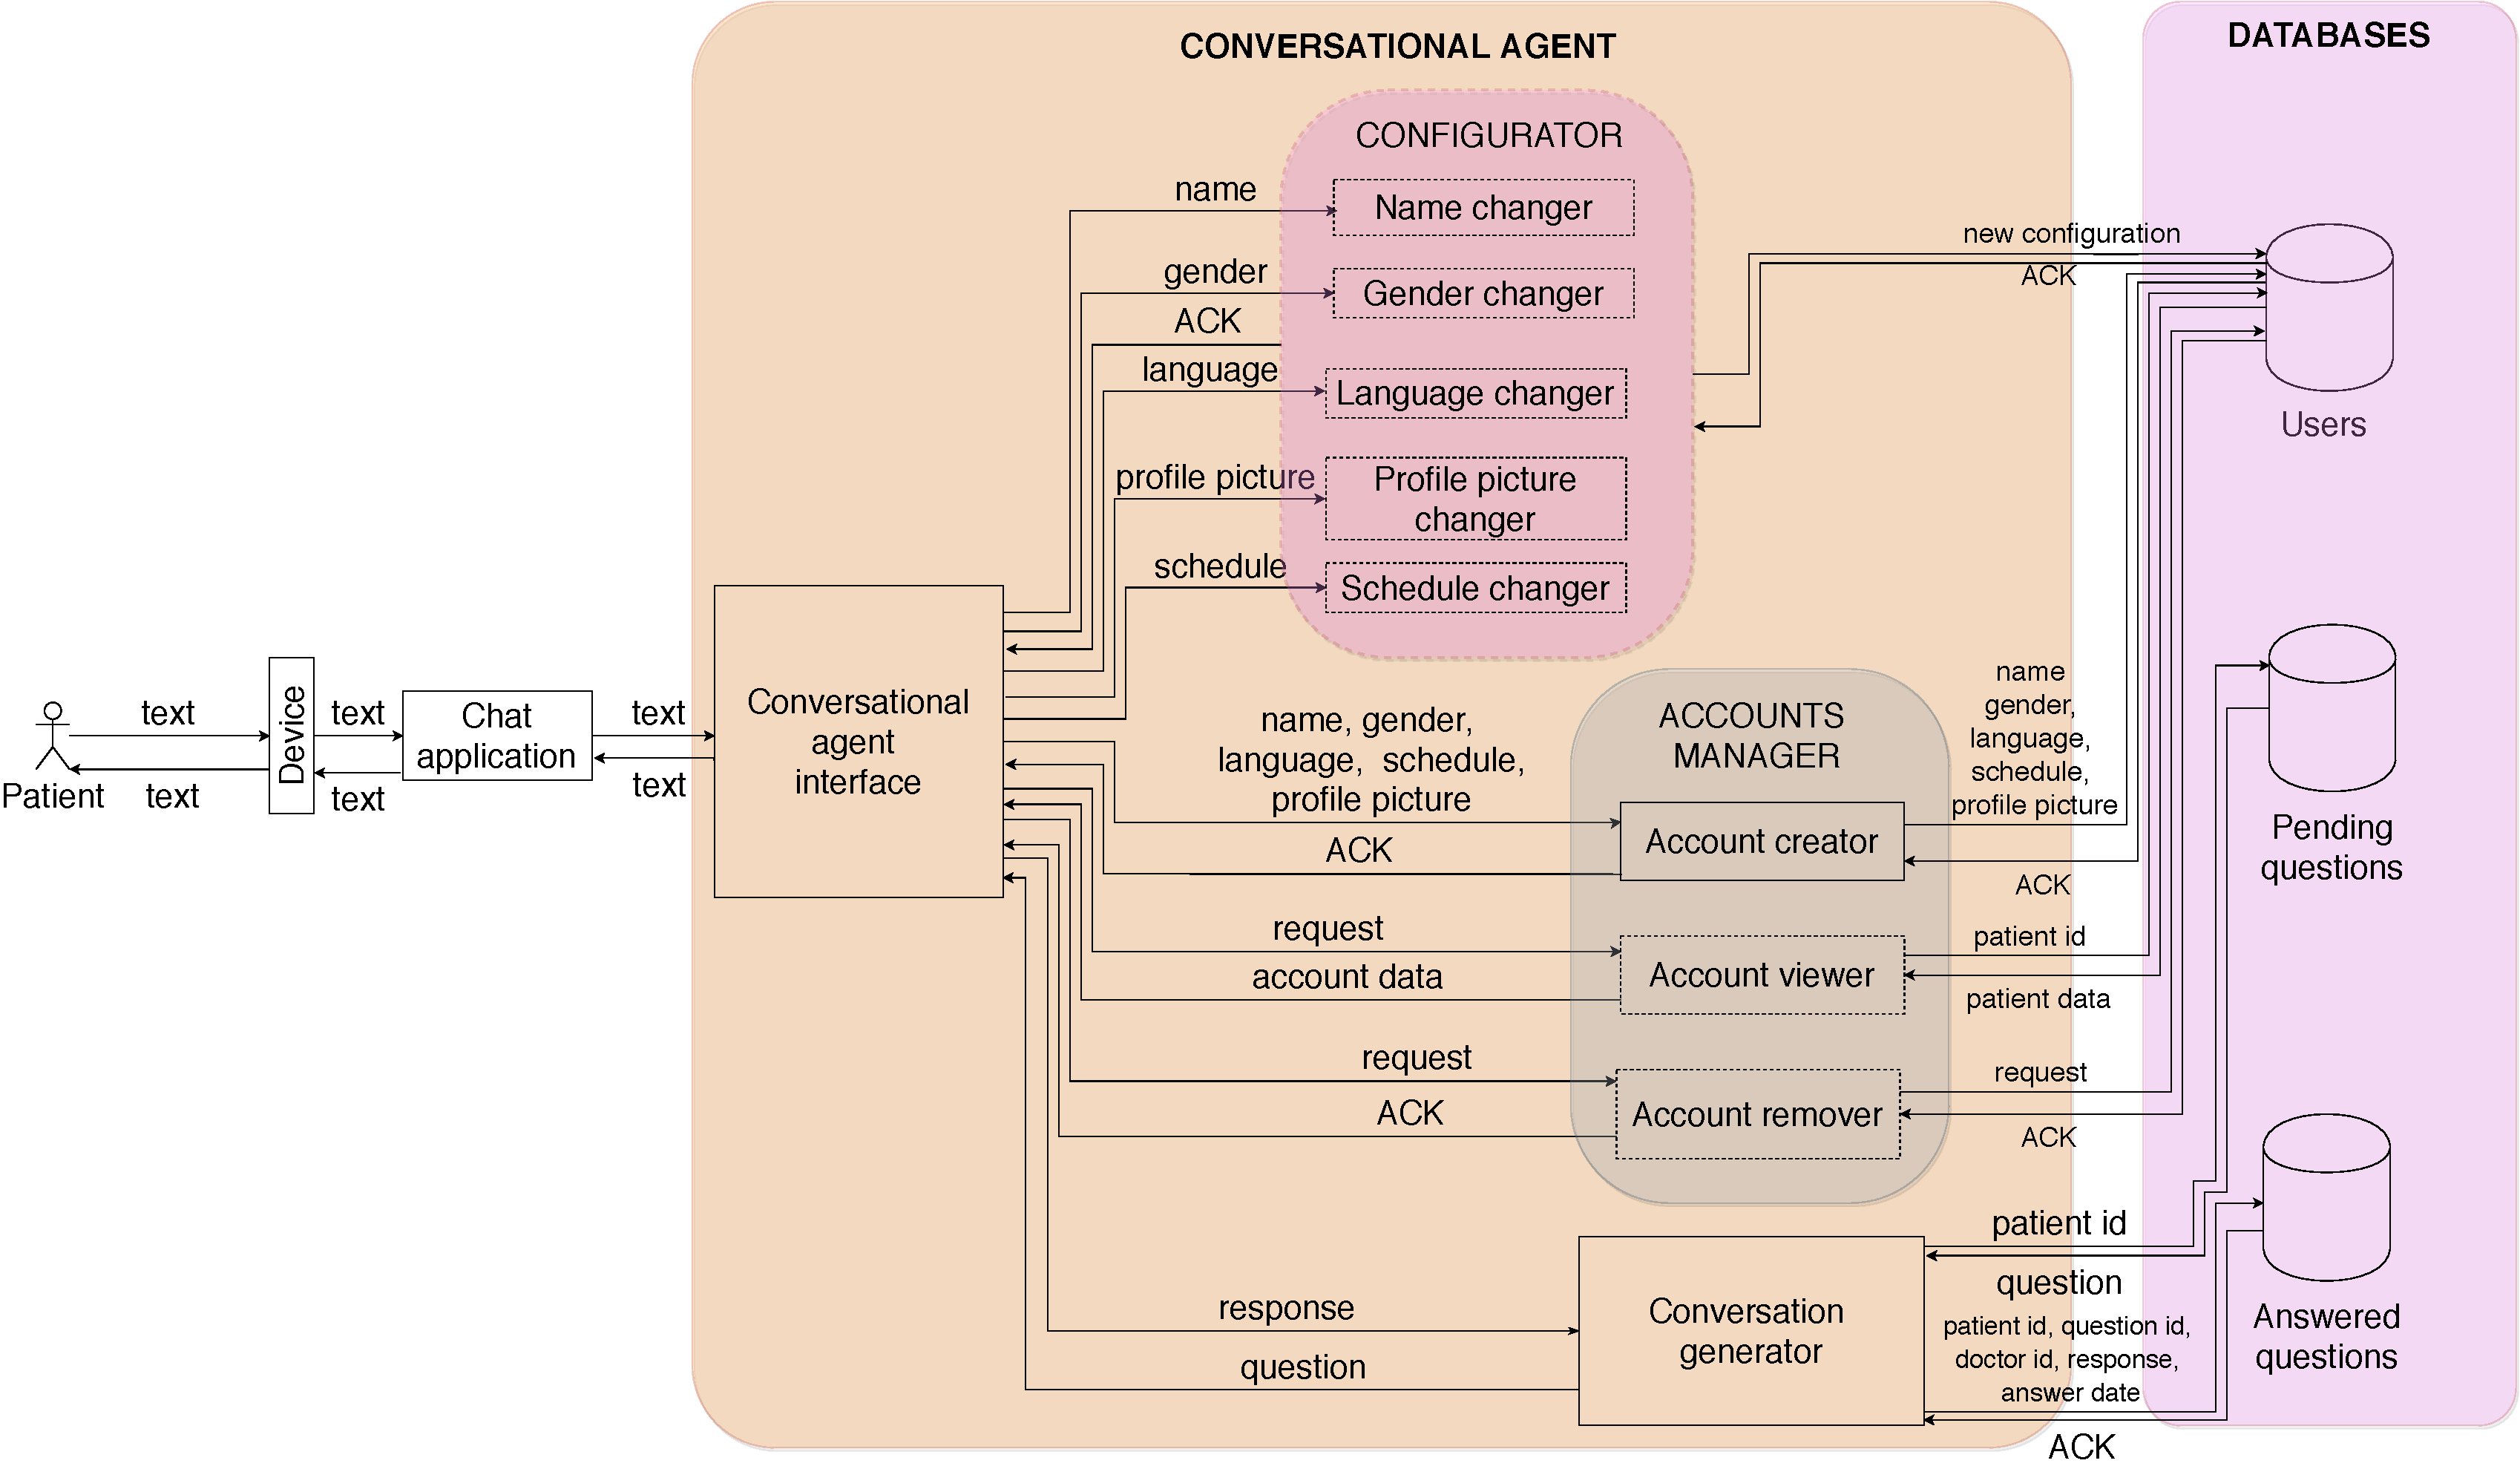
\includegraphics[width=\textwidth]{conv_agent.pdf}
    \caption{System architecture (conversational agent and databases).}
\end{figure}
\end{frame}

\begin{frame}[fragile]{Architecture}
\begin{figure}[H]
    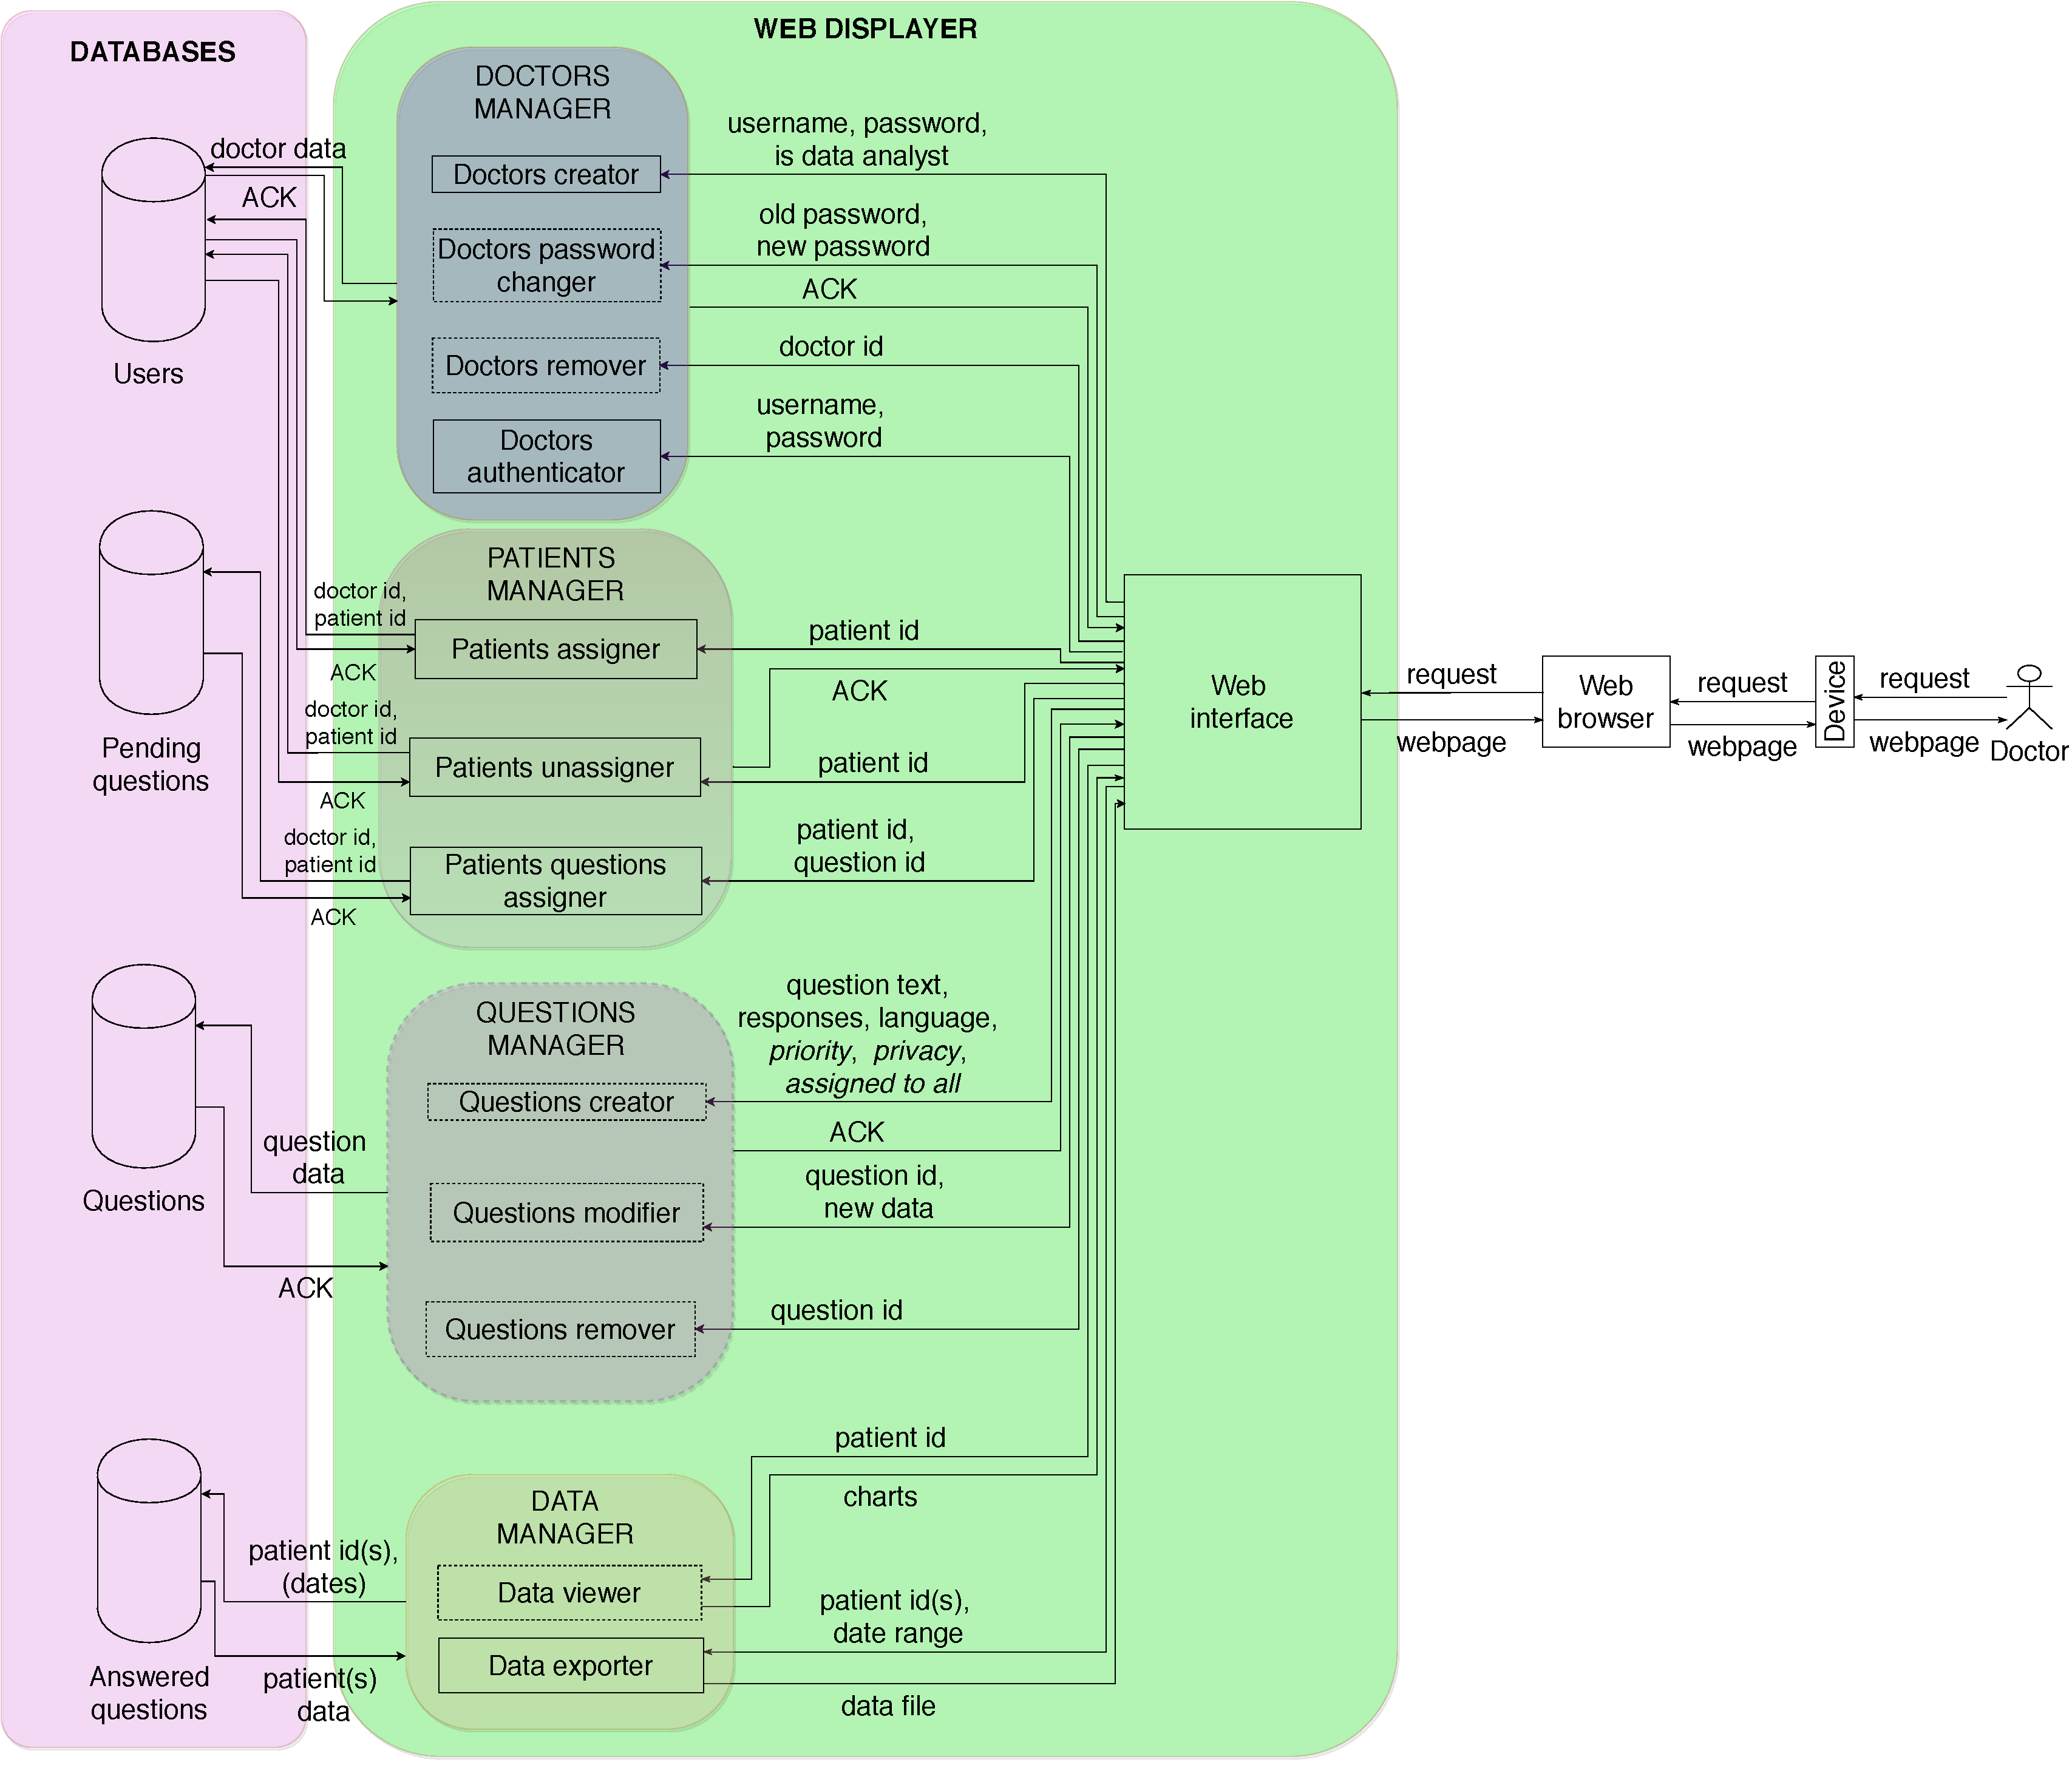
\includegraphics[width=0.75\textwidth]{web_int.pdf}
    \caption{System architecture (web interface and databases).}
\end{figure}
\end{frame}

\subsection{Implementation}

%%%%%%%%%%%%%%%%%%%%%%%%%%%%%

\begin{frame}[fragile]{Implementation (databases)}
  \begin{figure}[H]
    \centering
      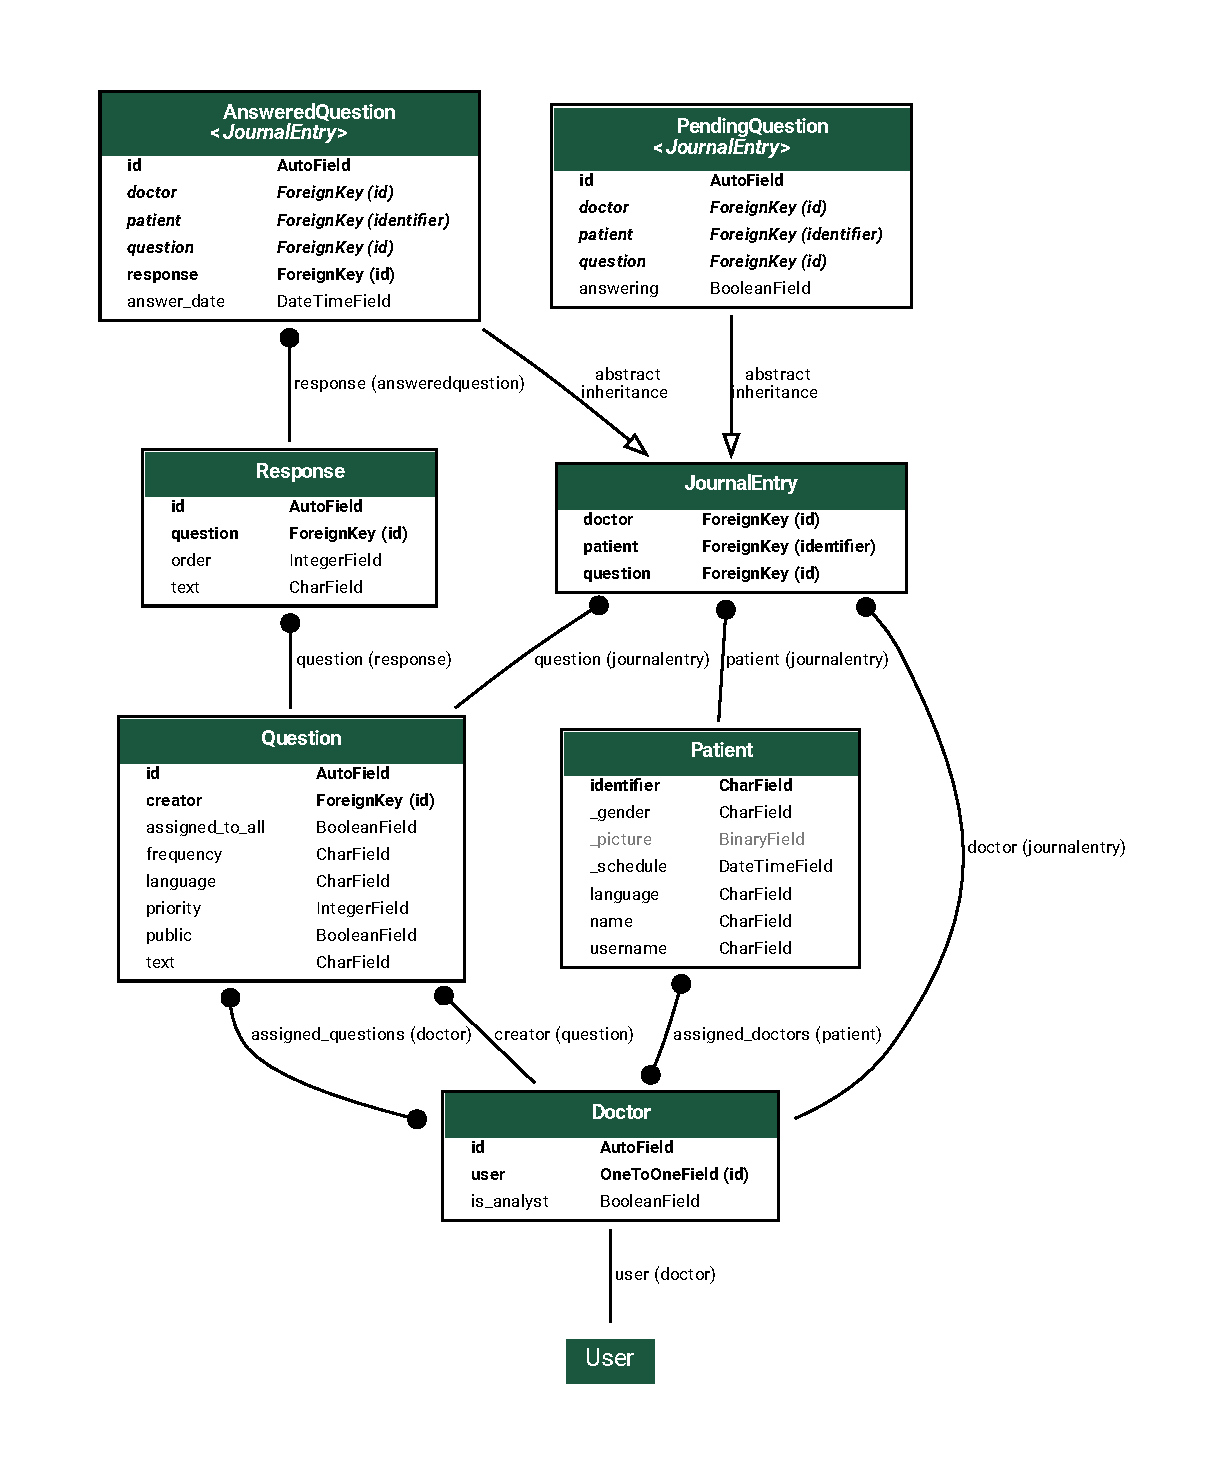
\includegraphics[width=0.55\textwidth]{class_diagram_zoom.pdf}
      \caption{System class diagram (HOW-R-U classes).}
  \end{figure}
\end{frame}

\begin{frame}[fragile]{Implementation (conversational agent)}
  \begin{itemize}[<+->]
    \item Handlers.
          \begin{itemize}[<+->]
            \item Start handler
            \item Config handler.
            \item Question handler.
          \end{itemize}
        \item Jobs.
          \begin{itemize}[<+->]
            \item PendingQuestionJob
          \end{itemize}
  \end{itemize}
\end{frame}

\begin{frame}[fragile]{Implementation (conversational agent start handler)}
  \begin{minted}[fontsize=\tiny, breaklines]{python}
  GENDER, PICTURE, LANGUAGE, SCHEDULE = range(4)
  @send_typing_action
  def start(update, context):
      """
      Shows welcome message and asks for language
      """
      # Check that user is not registered
      try:
          patient = Patient.objects.get(identifier=update.message.from_user.id)
          logger.info(  f'User {update.message.from_user.username} tried to register again.')
          update.message.reply_text(text=messages[patient.language]['already_exists'])
          return ConversationHandler.END
      except Patient.DoesNotExist:
          # The user should not exist in DB
          context.user_data['patient'] = Patient(name=update.message.from_user.first_name, identifier=str(update.message.from_user.id), username=update.message.from_user.username)
          logger.info(f'User {update.message.from_user.username} started a new conversation')
          send_welcome_message(patient)
          send_language_selection(patient)
      return LANGUAGE
\end{minted}
\end{frame}

\begin{frame}[fragile]{Implementation (conversational agent start handler)}
  \begin{minted}[fontsize=\tiny, breaklines]{python}
  start_handler = ConversationHandler(
      entry_points=[CommandHandler('start', start)],
      states={
          LANGUAGE: [MessageHandler(Filters.regex(f'^({Flag.flag("es")}|{Flag.flag("gb")})$'), language)],
          GENDER: [MessageHandler(Filters.regex('^(Male|Female|Other|Masculino|Femenino|Otro)$'), gender)],
          PICTURE: [MessageHandler(Filters.photo, picture), CommandHandler('skip', skip_picture)],
          SCHEDULE: [MessageHandler(Filters.regex('^([0-1]?[0-9]|2[0-3]):[0-5][0-9]$'), schedule)]
      },
      fallbacks=[]
  )
\end{minted}
\end{frame}
%%%%%%%%%%%%%%%%%%%%%%%%%%%%%%%%%%%%%%%%%%%%%%%%%%%%%
\begin{frame}[fragile]{Implementation (conversational agent PendingQuestionJob)}
  \begin{minted}[fontsize=\tiny, breaklines]{python}
  class PendingQuestionJob(object):

    def __init__(self, context, patient):
        self.patient = patient
        self._create_job(context)

    def _create_job(self, context):
        context.job_queue.run_daily(callback=self.job_callback, time=self.patient.schedule, name=f'{self.patient.identifier}_pending_questions_job')

    def job_callback(self, context):
        pending_questions = self._get_pending_questions()
        for task in pending_questions:
            if not self.is_question_answered(task):
              task.answering = True
              ask_question(task, self.patient)
        send_message(self.patient, "All questions have been answered")
        if was_configurator_running(self.patient.identifier, context):
          reopen_configurator(self.patient)
\end{minted}
\end{frame}
%%%%%%%%%%%%%%%%%%%%%%%%
\begin{frame}[fragile]{Implementation (conversational agent)}
  \begin{figure}[H]
    \centering
      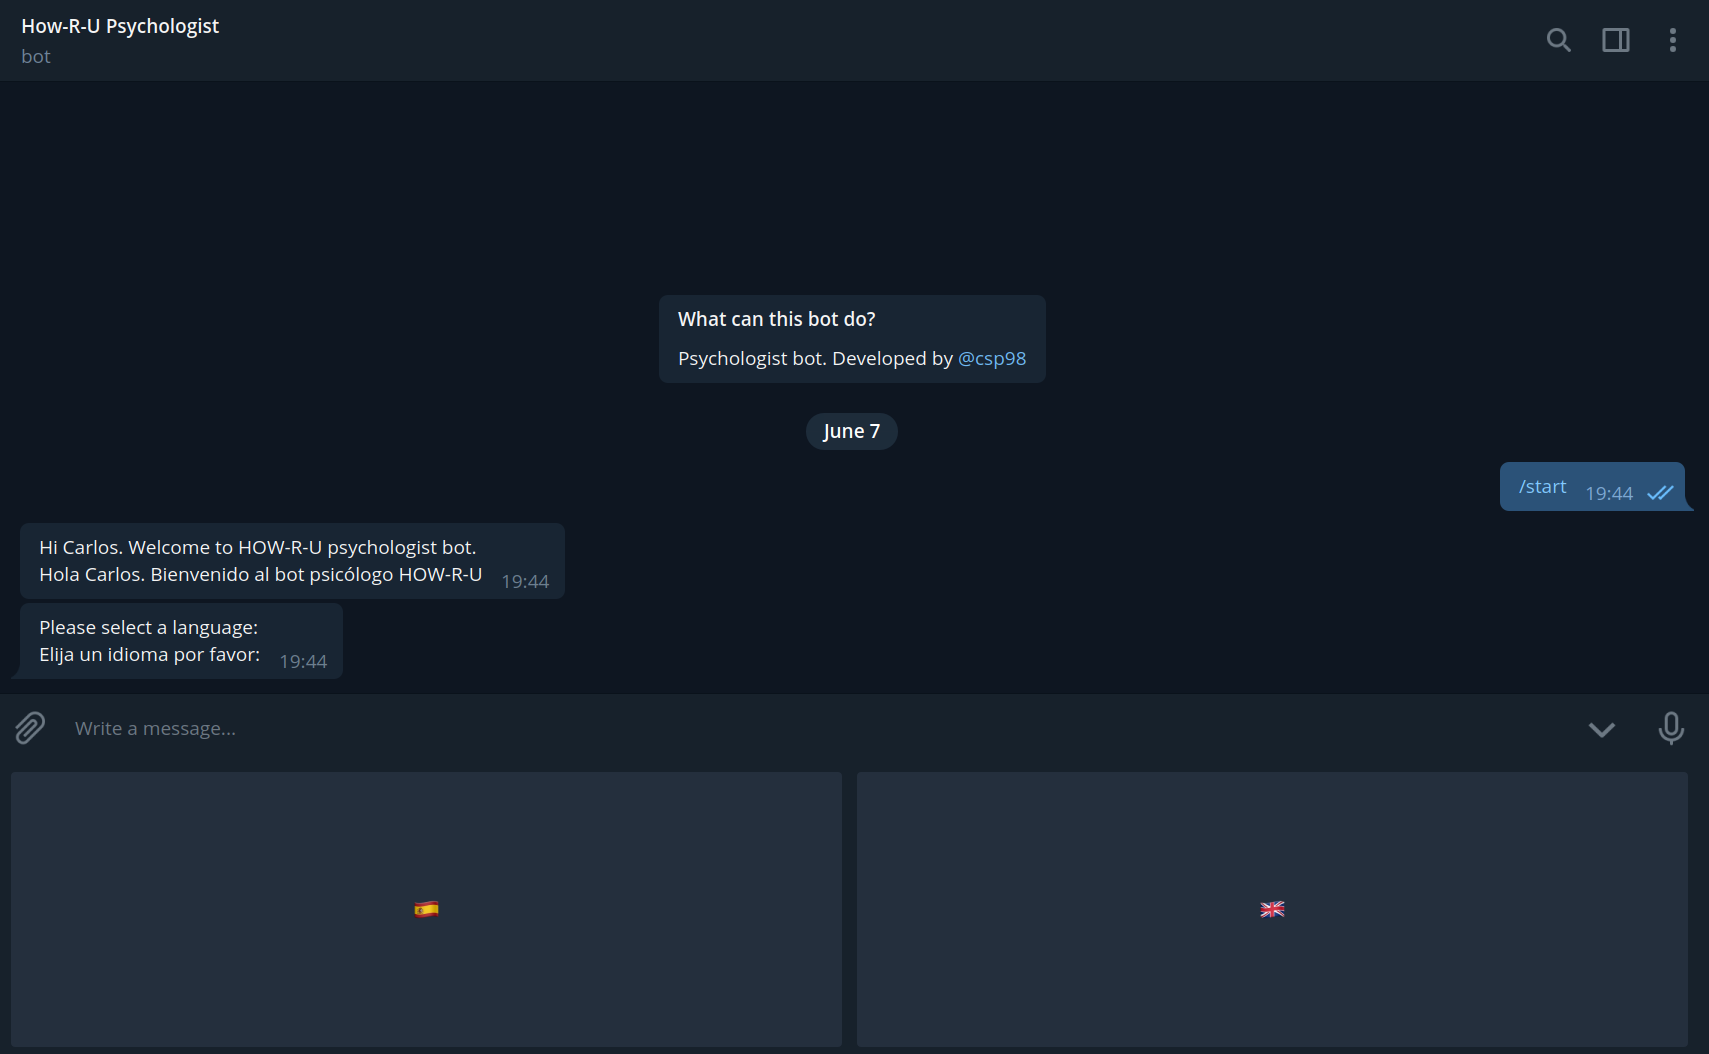
\includegraphics[width=0.35\textwidth]{start.png}
      \caption{Agent showing the welcome message and asking for language selection.}
  \end{figure}
\end{frame}
%%%%%%%%%%%%%%%%%%%%%%
\begin{frame}[fragile]{Implementation (conversational agent)}
  \begin{figure}[H]
    \centering
      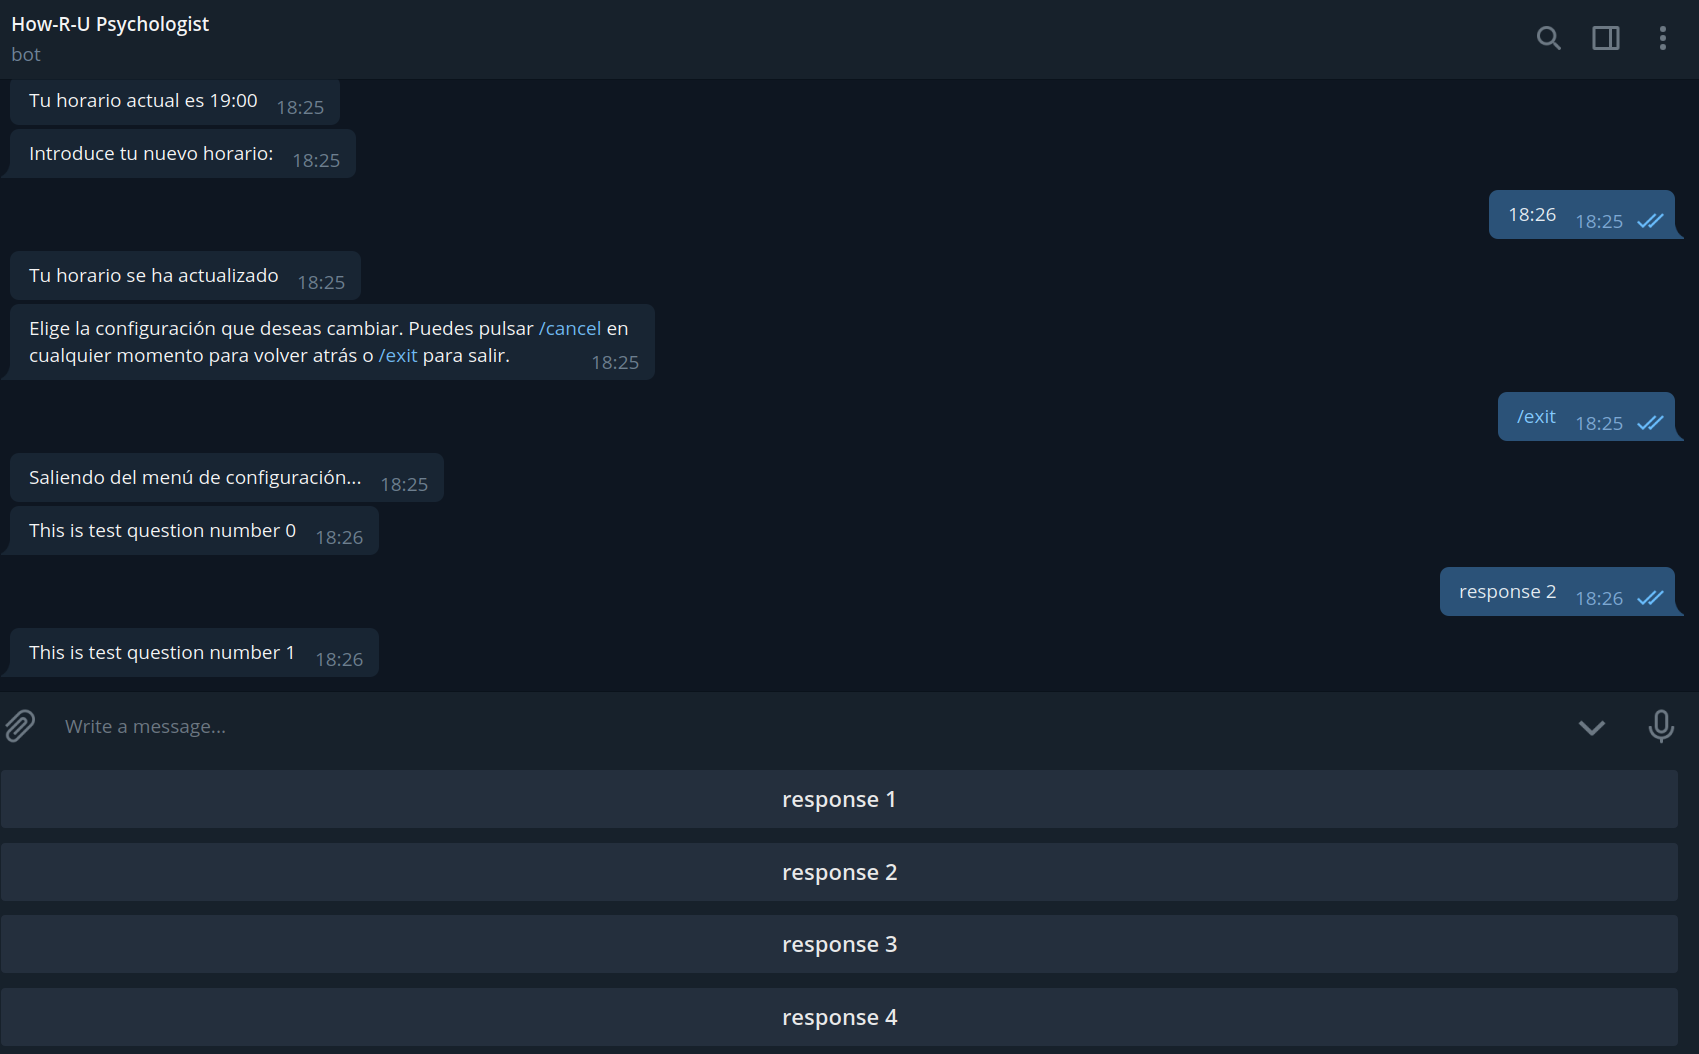
\includegraphics[width=\textwidth]{bot_answering.png}
    \caption{HOW-R-U converstional agent asking a question to a patient.}
  \end{figure}
\end{frame}
%%%%%%%%%%%%%%%%%%%%%%%%%%%%

\begin{frame}[fragile]{Implementation (web interface)}
  \begin{figure}[H]
      \centering
      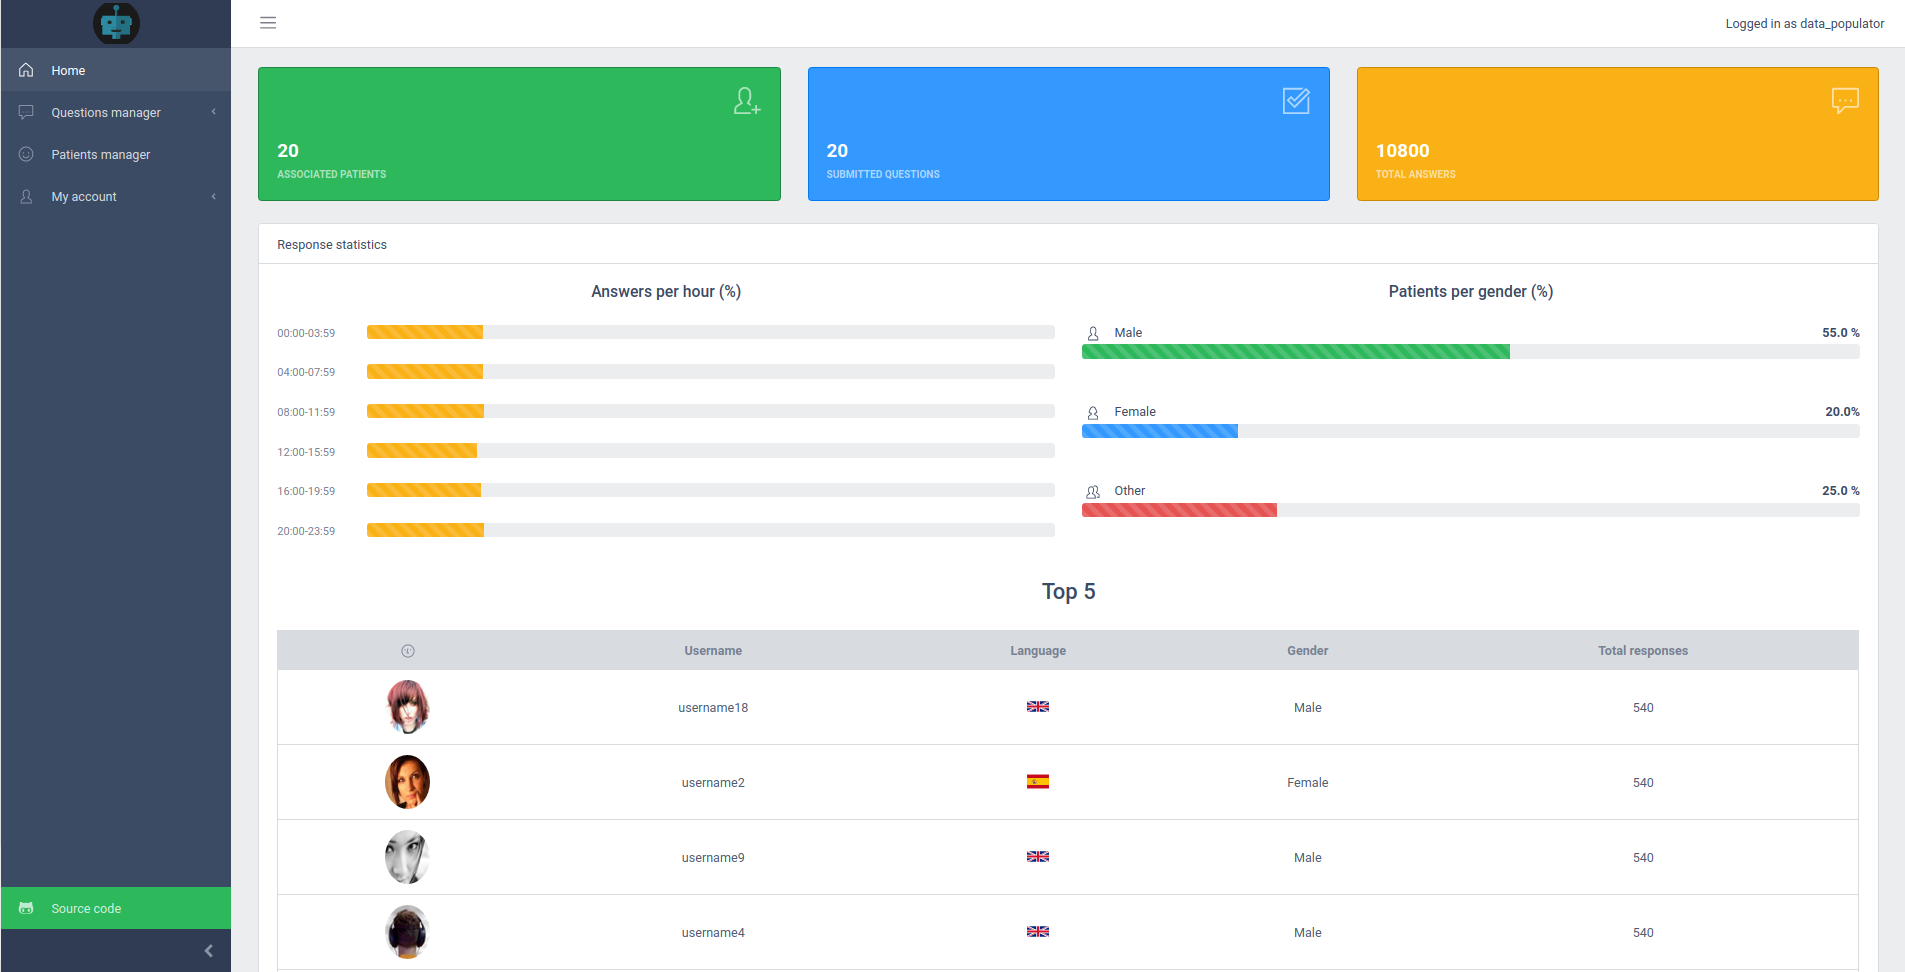
\includegraphics[width=\textwidth]{homepage.png}
      \caption{HOW-R-U homepage.}
  \end{figure}
\end{frame}
%%%%%%%%%%%%%%%%%%%%%%%%%%

\begin{frame}[fragile]{Implementation (web interface)}
  \begin{minted}[fontsize=\tiny, breaklines]{python}
    @login_required(login_url="/login/")
    def index(request):
        """
        Shows the index page, including global parameters (top patients, number of associated patients, answers, gender and time percentages, etc.,)
        """
        doctor = request.user.doctor
        top_patients = get_top_patients(doctor)
        doctor_patients = doctor.patient_set
        number_associated_patients = doctor_patients.count()
        submitted_questions = Question.objects.filter(creator=doctor).count()
        total_answers = get_total_answers(doctor)
        male_percentage, female_percentage, other_percentage = get_gender_stats(doctor, number_associated_patients)
        answers_per_hour = get_answers_per_hour(doctor)
        context = {
            "top_patients": top_patients,
            "number_associated_patients": number_associated_patients,
            "submitted_questions": submitted_questions,
            "total_answers": total_answers,
            "male_percentage": male_percentage,
            "female_percentage": female_percentage,
            "other_percentage": other_percentage,
            "answers_per_hour": answers_per_hour
        }
        return render(request, "index.html", context)
  \end{minted}
\end{frame}

\begin{frame}[fragile]{Implementation (web interface)}
  \begin{figure}[H]
      \centering
      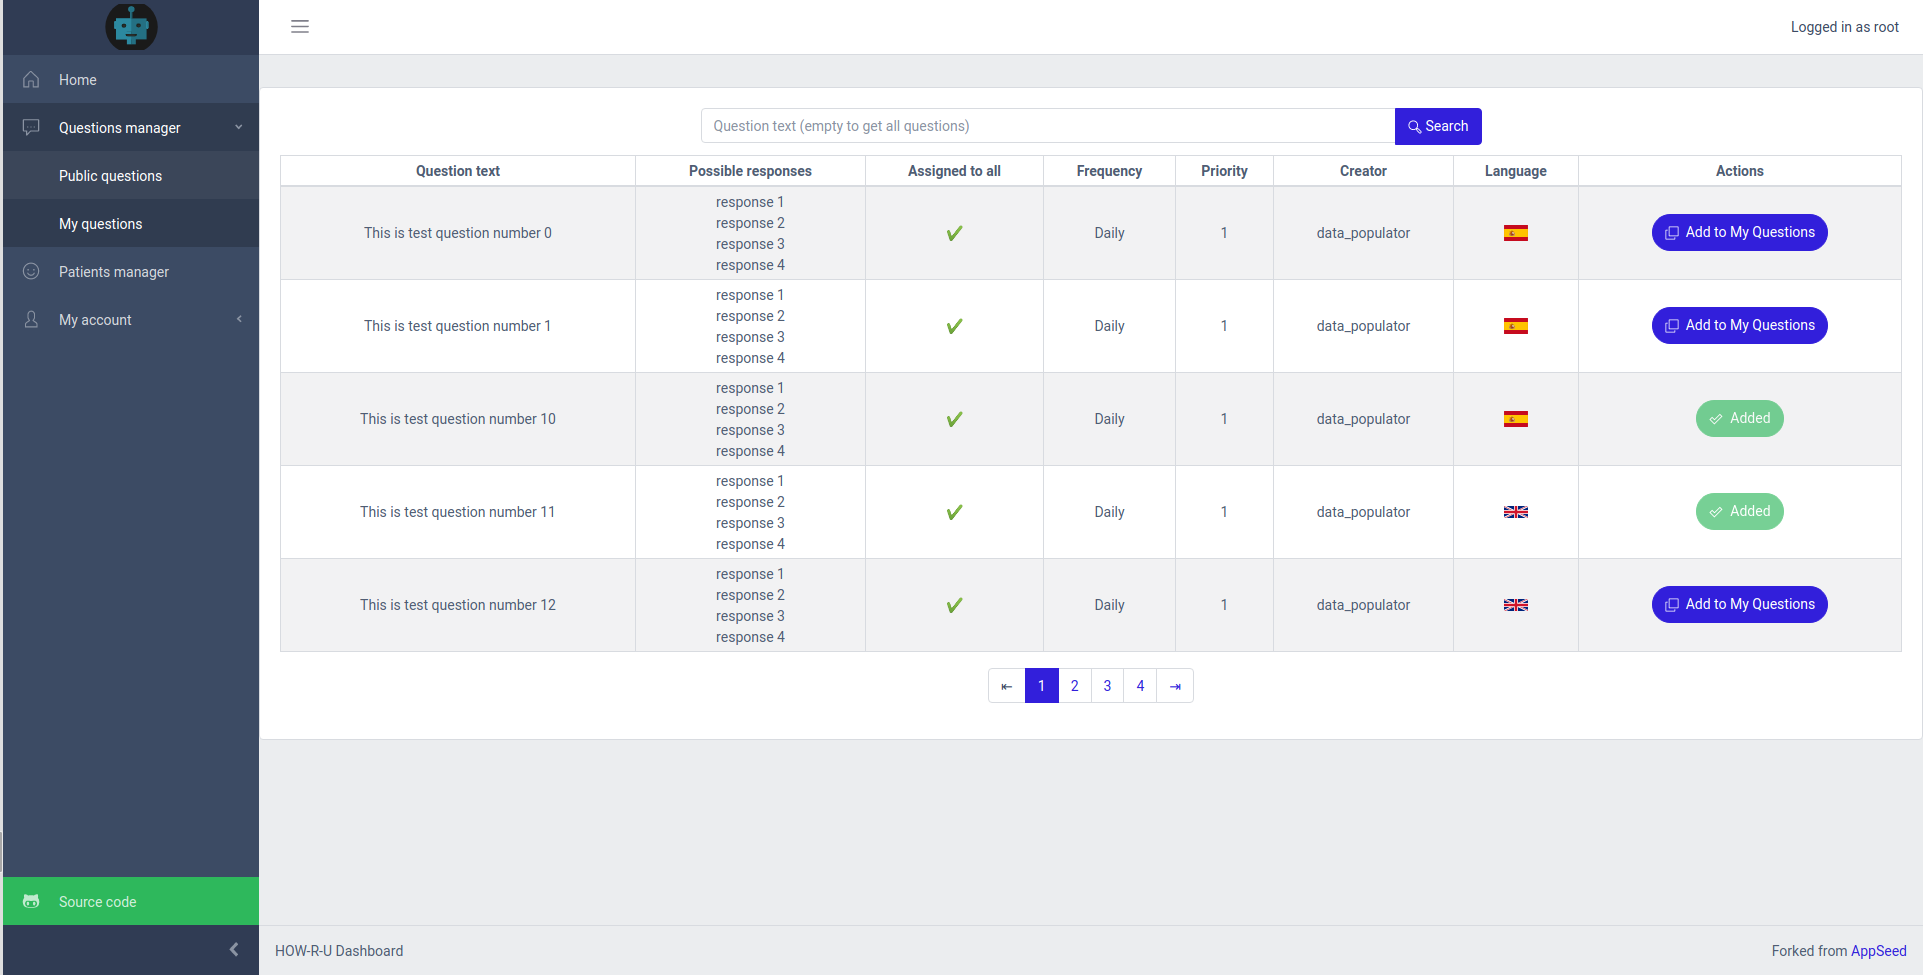
\includegraphics[width=\textwidth]{public_questions.png}
      \caption{Public questions page.}
  \end{figure}
\end{frame}
%%%%%%%%%%%%%%%%%%%%%%%%%%%%%%%%%%%%
\begin{frame}[fragile]{Implementation (web interface)}
  \begin{figure}[H]
    \centering
      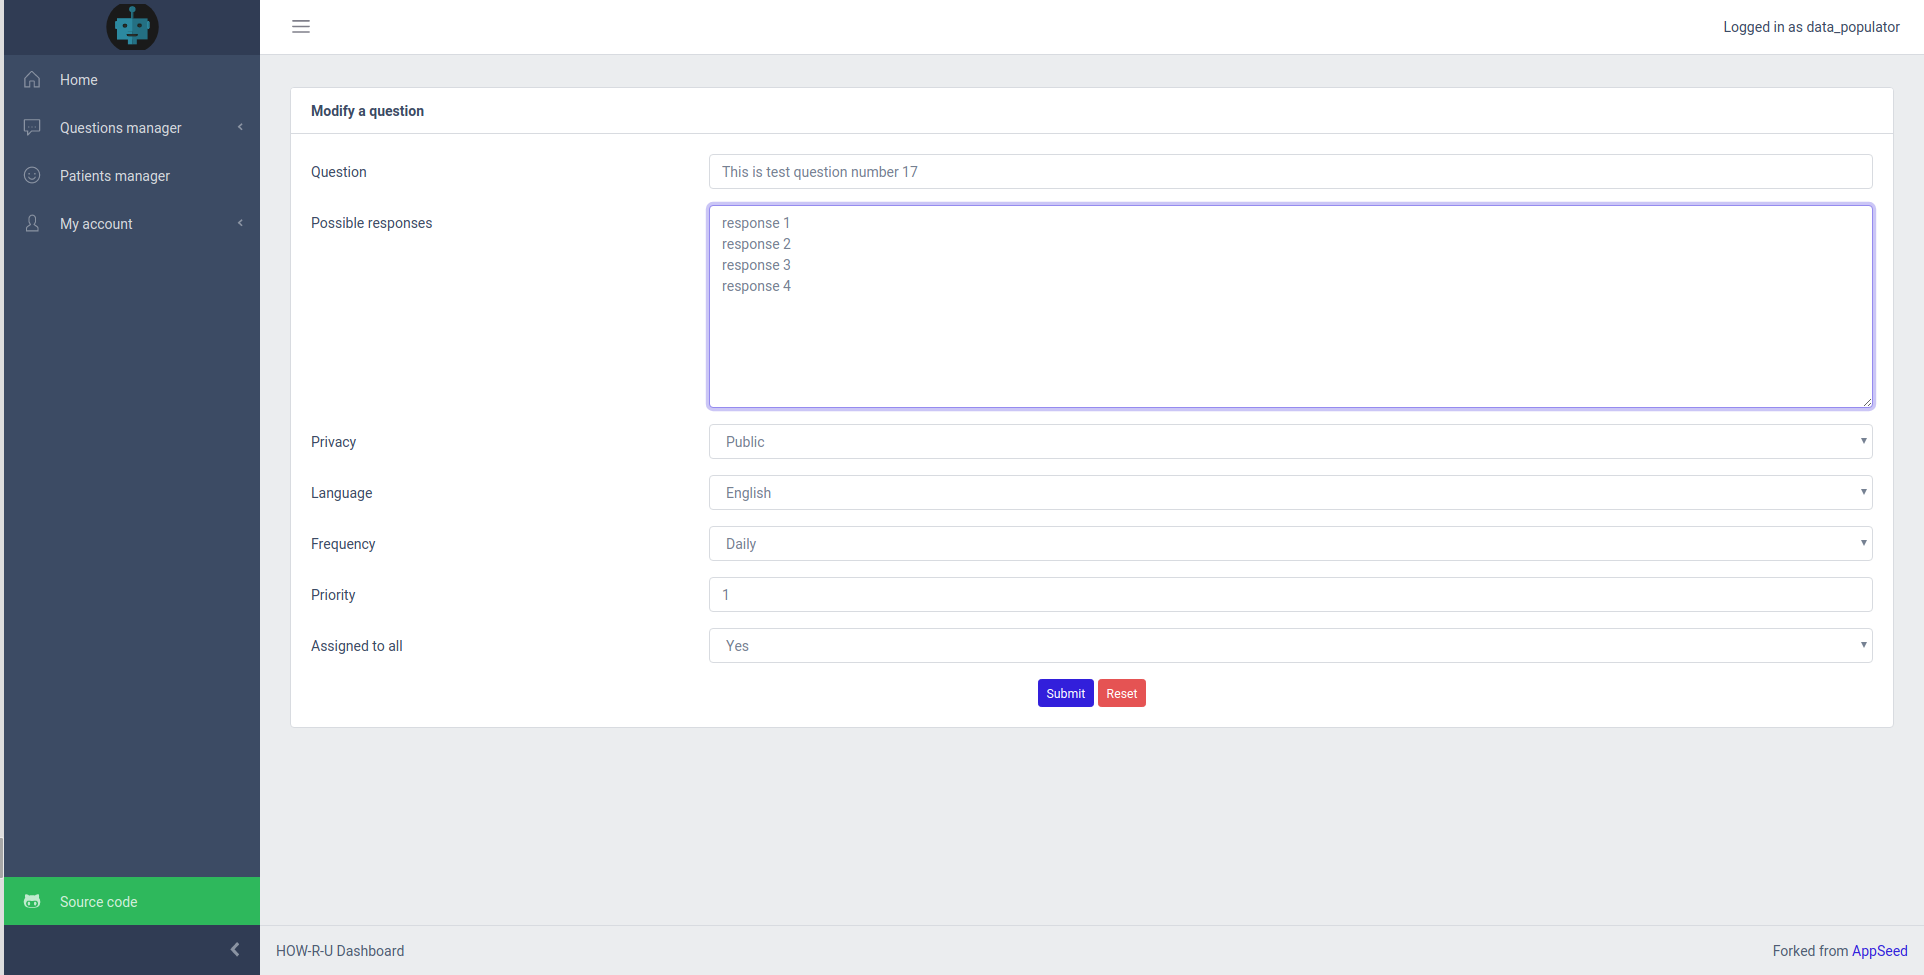
\includegraphics[width=\textwidth]{questions_modifier.png}
    \caption{Questions creator and modifier.}
  \end{figure}
\end{frame}
%%%%%%%%%%%%%%%%%%%%%%%%%%%%%%%%%%%%
\begin{frame}[fragile]{Implementation (web interface)}
  \begin{figure}[H]
    \centering
      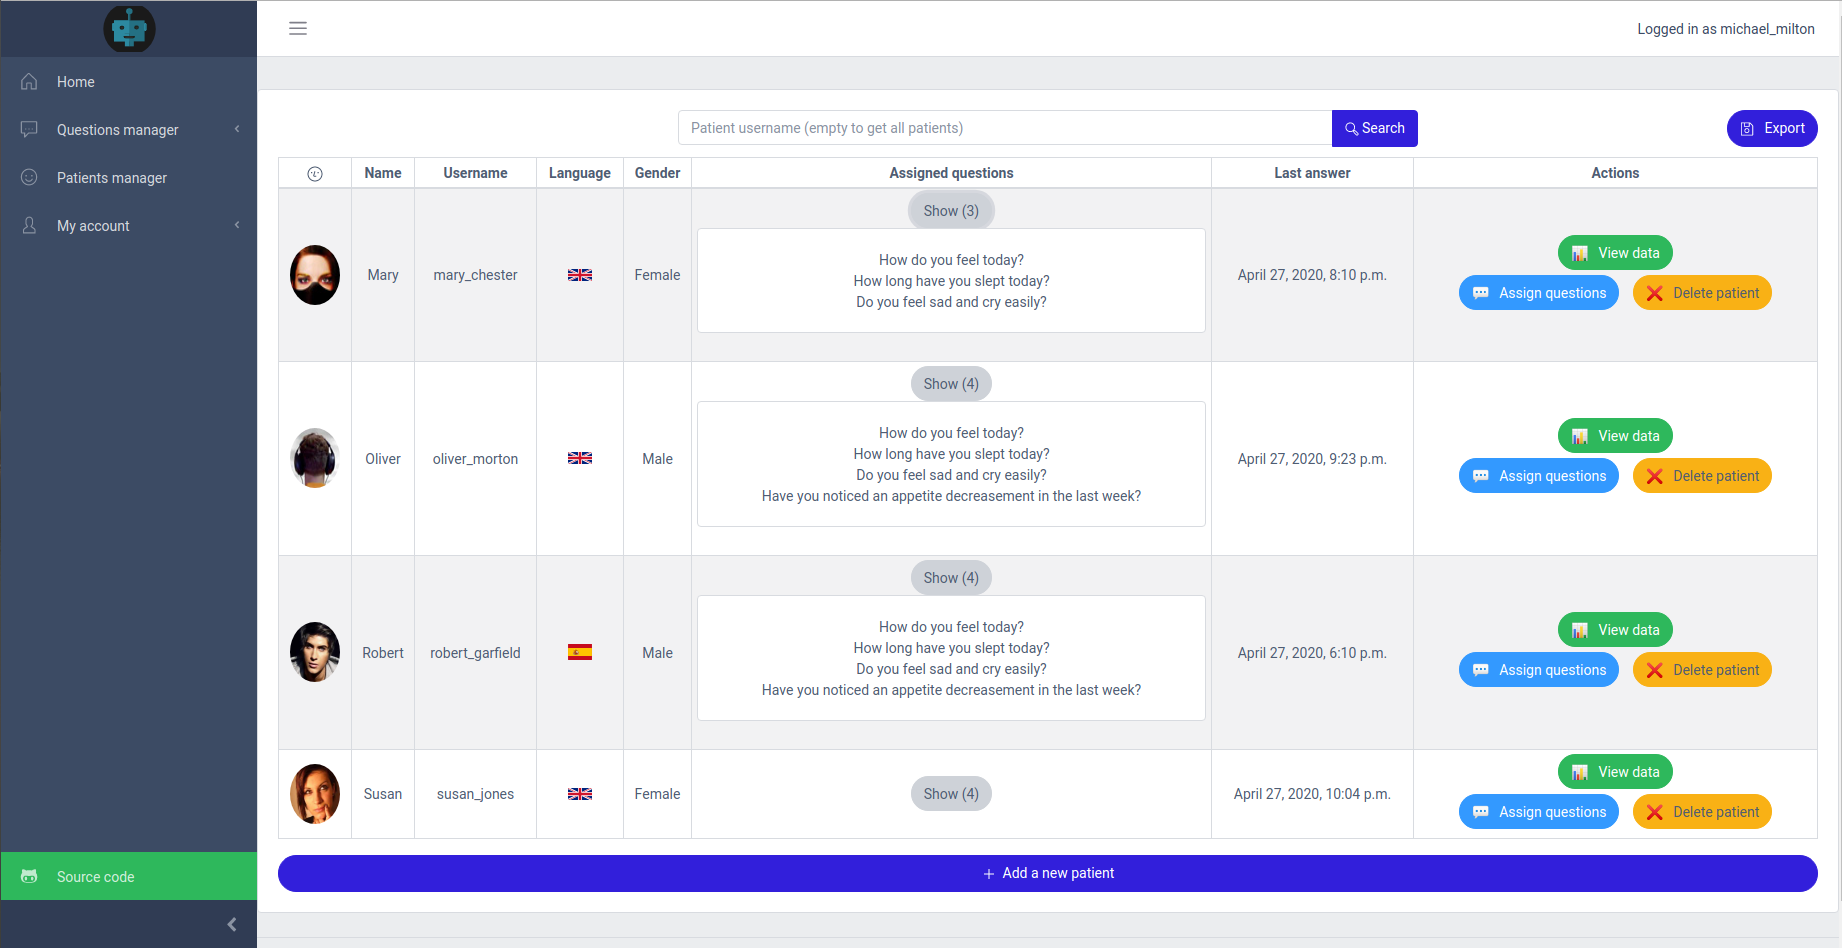
\includegraphics[width=\textwidth]{patients_manager.png}
    \caption{Patients manager.}
  \end{figure}
\end{frame}
%%%%%%%%%%%%%%%%%%%%%%%%%%%%%%%%%%%%
\begin{frame}[fragile]{Implementation (web interface)}
  \begin{figure}[H]
    \centering
      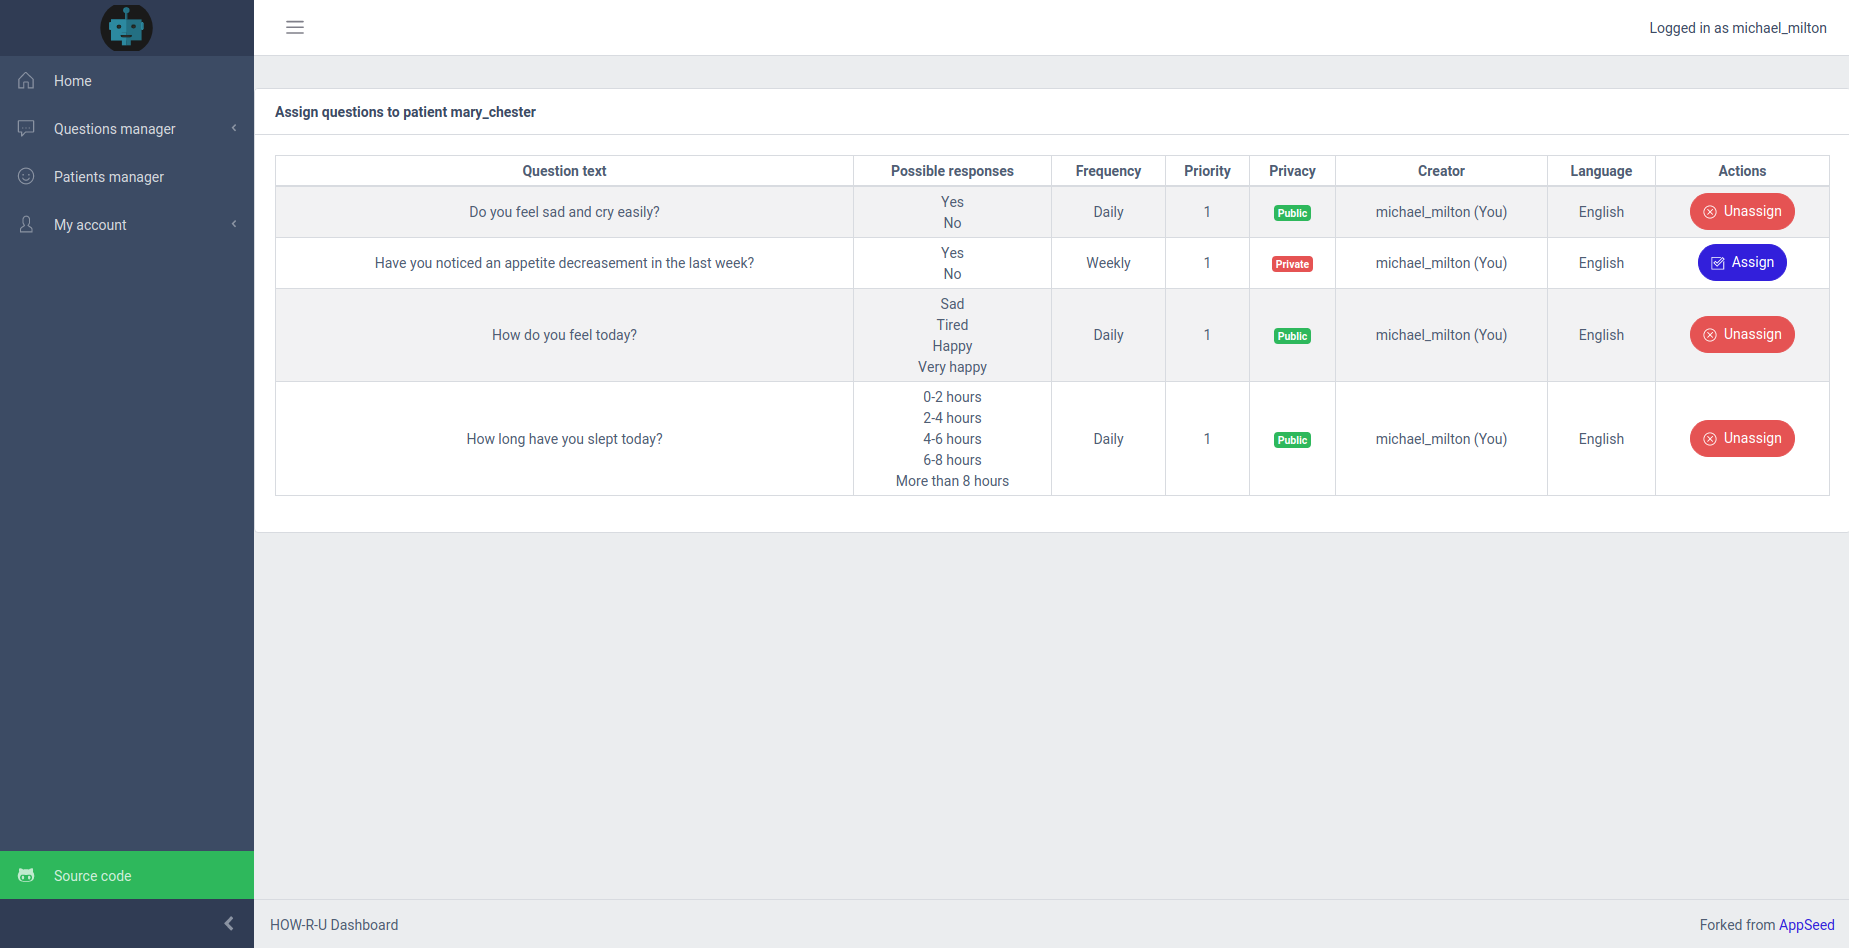
\includegraphics[width=\textwidth]{assign_questions.png}
    \caption{Patients manager assign questions page.}
  \end{figure}
\end{frame}
%%%%%%%%%%%%%%%%%%%%%%%%%%%%%%%%%%%%
\begin{frame}[fragile]{Implementation (web interface)}
  \begin{figure}[H]
    \centering
      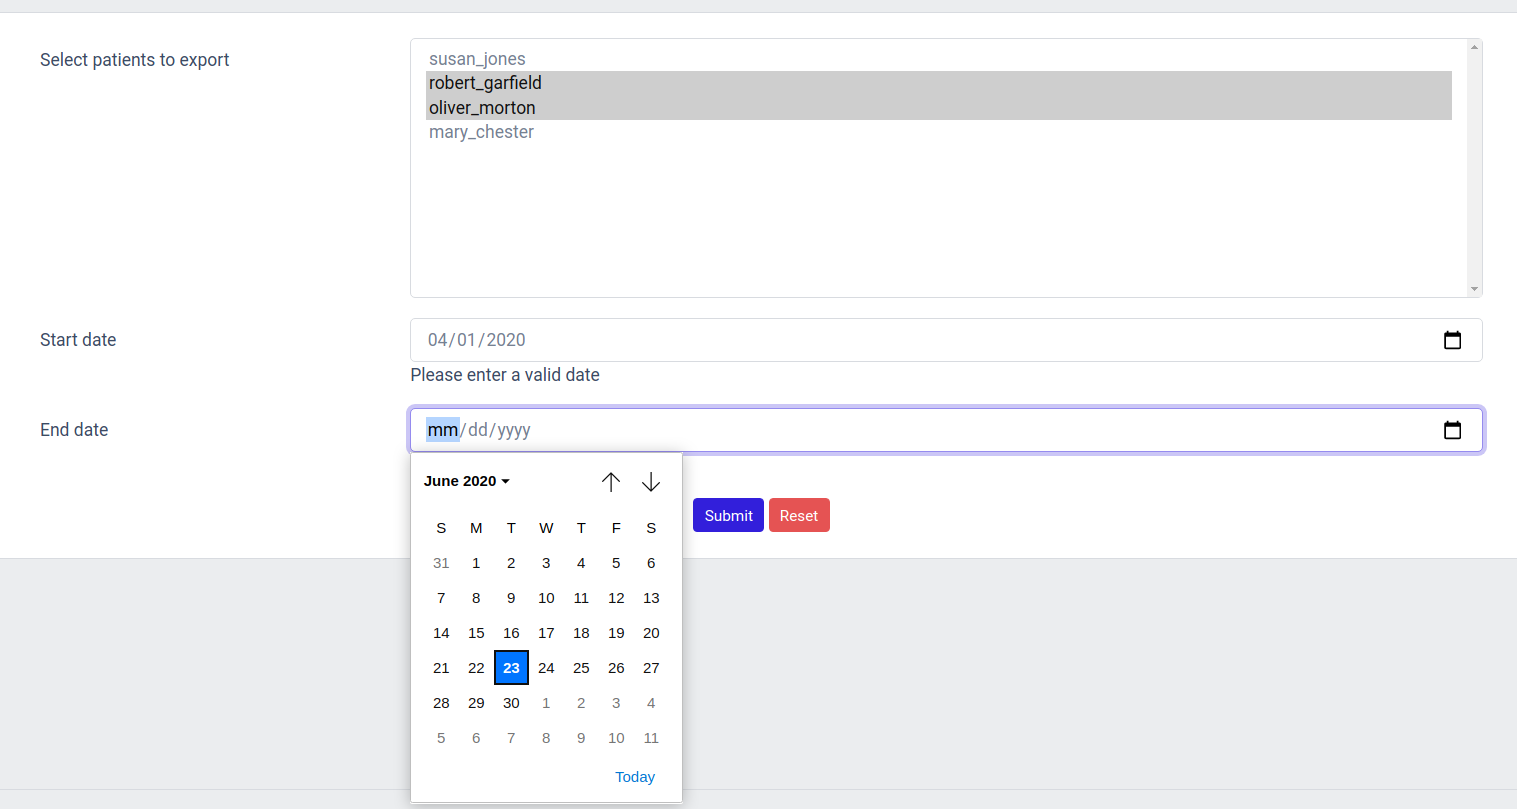
\includegraphics[width=\textwidth]{export.png}
    \caption{Export page}
  \end{figure}
\end{frame}
%%%%%%%%%%%%%%%%%%%%%%%%%%%%%%%%%%%%
\begin{frame}[fragile]{Implementation (web interface)}
  \begin{table}[h!]
  \centering
  \resizebox{\textwidth}{!}{%
  \begin{tabular}{@{}cccc@{}}
  \toprule
  \textbf{Patient username} & \textbf{Question}                                                                                      & \textbf{Answer}   & \textbf{Date}       \\ \midrule
  robert\_garfield          & How do you feel today?                                                                                 & Tired             & 2020-04-01 04:12:20 \\
  robert\_garfield          & How do you feel today?                                                                                 & Sad               & 2020-04-02 05:24:20 \\
  robert\_garfield          & How long have you slept today?                                                                         & 0-2 hours         & 2020-04-01 12:56:20 \\
  robert\_garfield          & How long have you slept today?                                                                         & 4-6 hours         & 2020-04-02 11:28:20 \\
  robert\_garfield          & Do you feel sad and cry easily?                                                                        & Yes               & 2020-04-01 14:22:21 \\
  robert\_garfield          & Do you feel sad and cry easily?                                                                        & No                & 2020-04-02 06:31:21 \\
  oliver\_morton            & How do you feel today?                                                                                 & Very happy        & 2020-04-01 01:45:19 \\
  oliver\_morton            & How do you feel today?                                                                                 & Happy             & 2020-04-02 02:59:19 \\
  oliver\_morton            & How long have you slept today?                                                                         & More than 8 hours & 2020-04-01 20:51:20 \\
  oliver\_morton            & How long have you slept today?                                                                         & 2-4 hours         & 2020-04-01 22:24:20 \\
  oliver\_morton            & Do you feel sad and cry easily?                                                                        & No                & 2020-04-01 07:47:20 \\
  oliver\_morton            & Do you feel sad and cry easily?                                                                        & Yes               & 2020-04-02 17:26:20 \\
  oliver\_morton            & \begin{tabular}[c]{@{}c@{}}Have you noticed an appetite \\ decreasement in the last week?\end{tabular} & Yes               & 2020-04-01 21:41:20 \\
  oliver\_morton            & \begin{tabular}[c]{@{}c@{}}Have you noticed an appetite \\ decreasement in the last week?\end{tabular} & Yes               & 2020-04-08 21:09:20 \\ \bottomrule
  \end{tabular}%
  }
  \caption{Example data generated with the \emph{Export} feature.}
  \end{table}
\end{frame}

%%%%%%%%%%%%%%%%%%%%%%%%%%%%%%%%%%%%
\begin{frame}[fragile]{Implementation (web interface)}
  \begin{figure}[H]
    \centering
      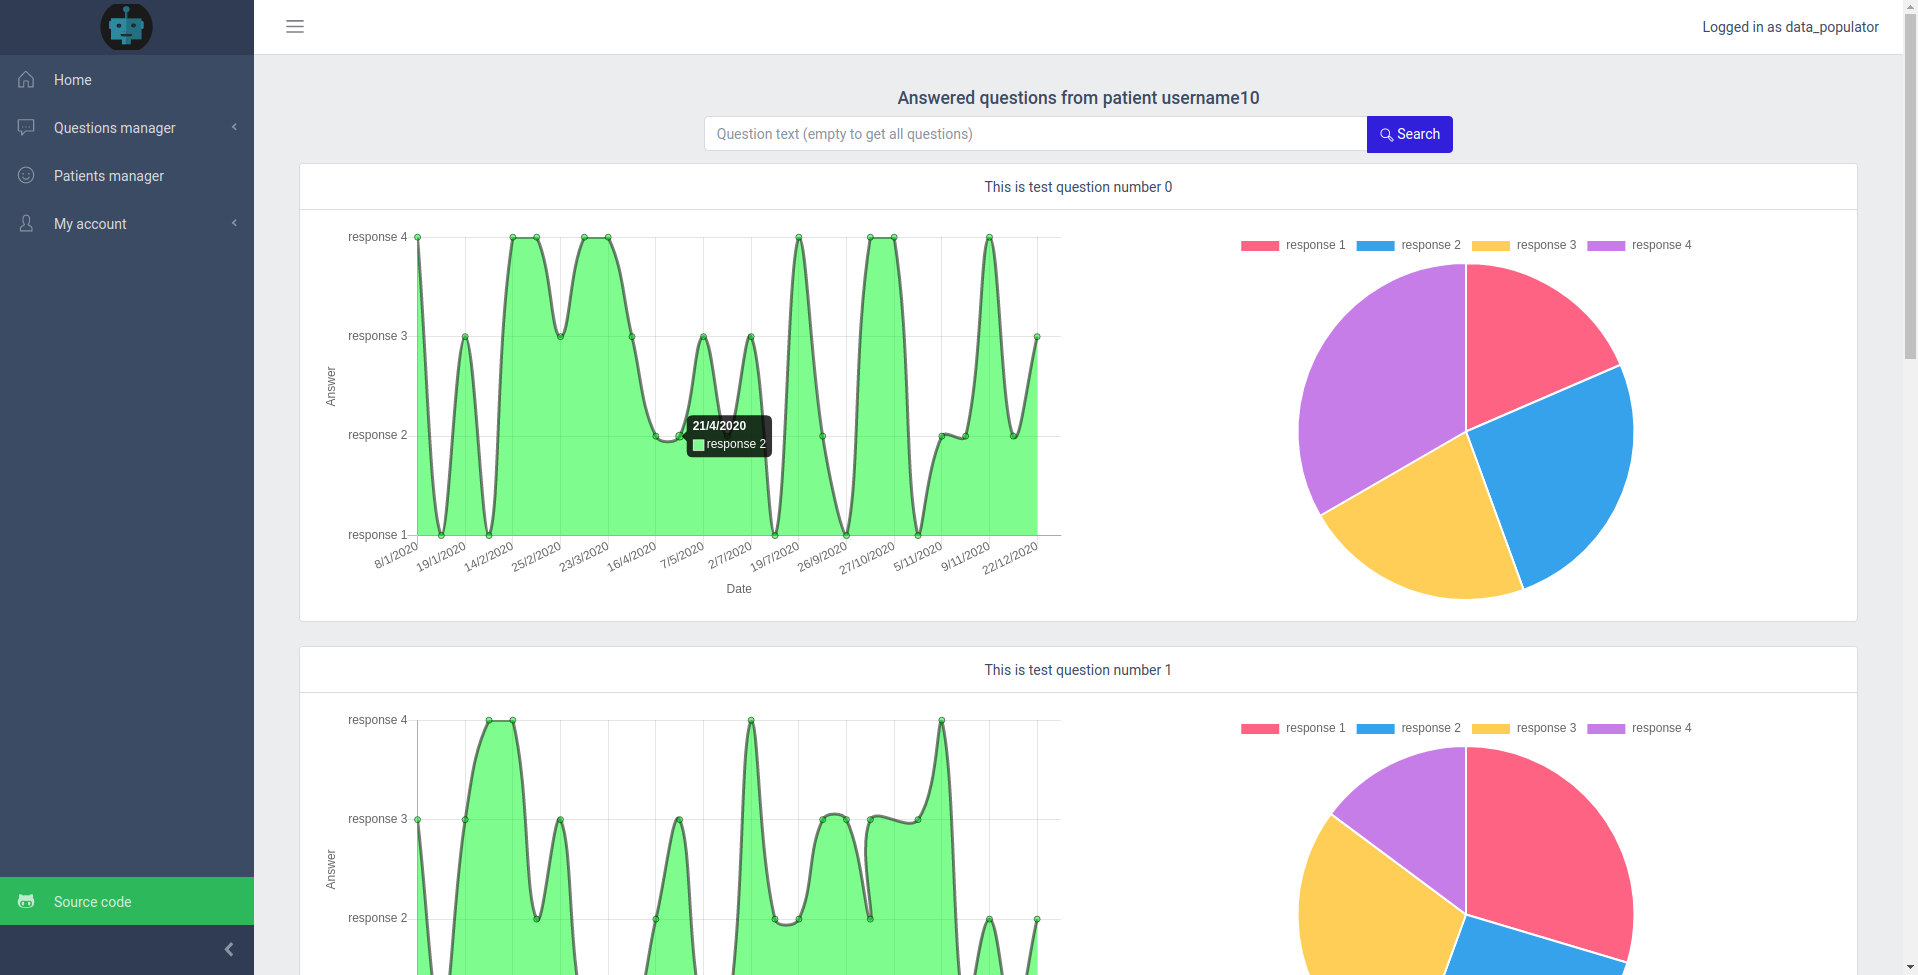
\includegraphics[width=\textwidth]{view_data.png}
    \caption{View data page.}
  \end{figure}
\end{frame}

\section{Environments}
\subsection{Development environment}
\begin{frame}[fragile]{Development environment}
  \begin{figure}[H]
    \centering
      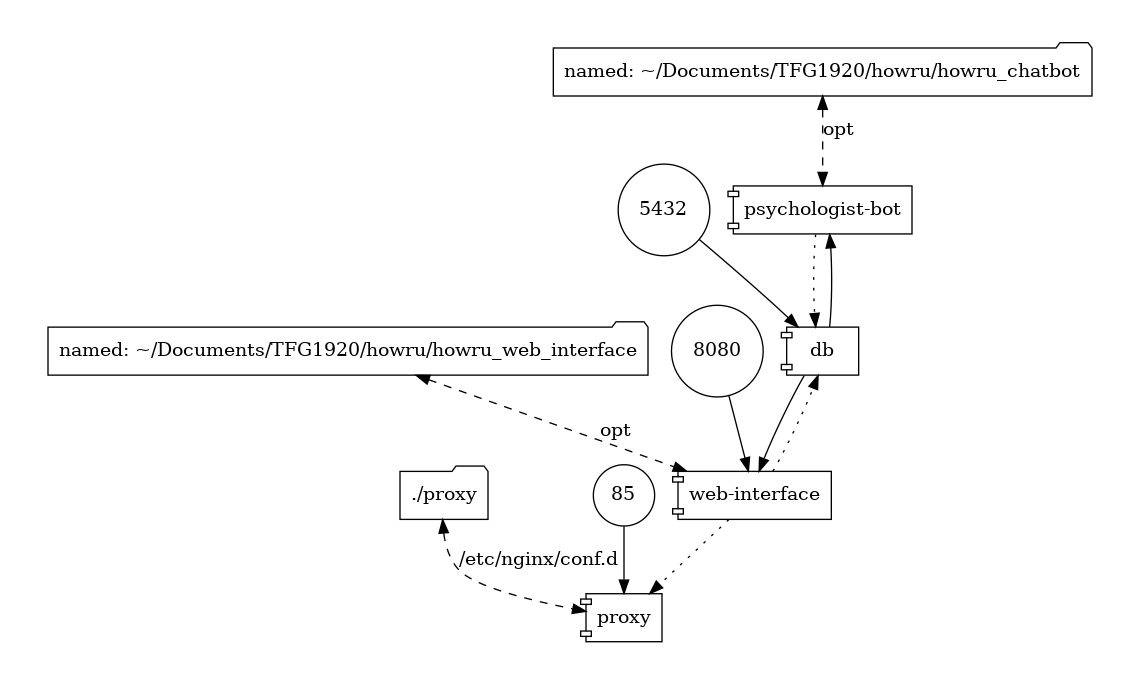
\includegraphics[width=\textwidth]{docker-compose.png}
      \caption{Docker-compose file schema. Generated by \protect\cite{dockerviz}.}
  \end{figure}
\end{frame}
\subsection{Production environments}
\begin{frame}[fragile]{Production scalable environment}
  \begin{figure}[H]
    \centering
    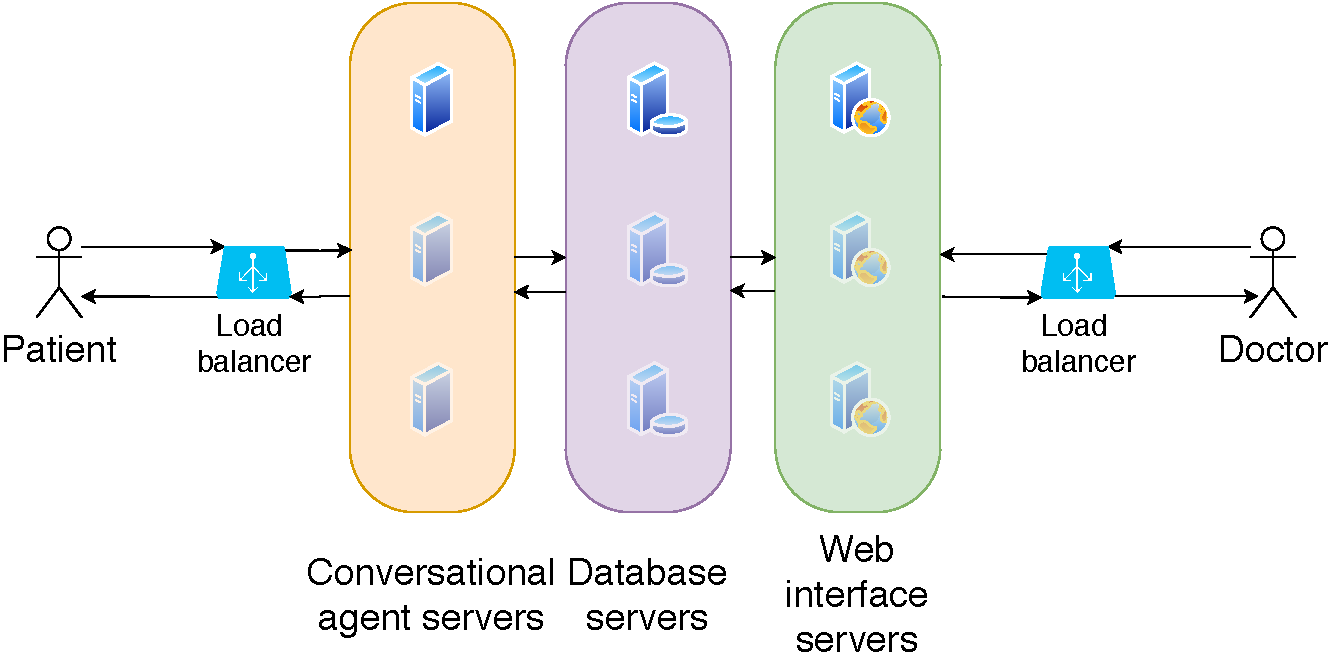
\includegraphics[width=0.7\textwidth]{scalable.pdf}
    \caption{Scalable environment architecture diagram. Created using \emph{diagrams.net} \protect\cite{drawio}.}
  \end{figure}
\end{frame}

\begin{frame}[fragile]{Production non-scalable environment}
  \begin{figure}[H]
    \centering
    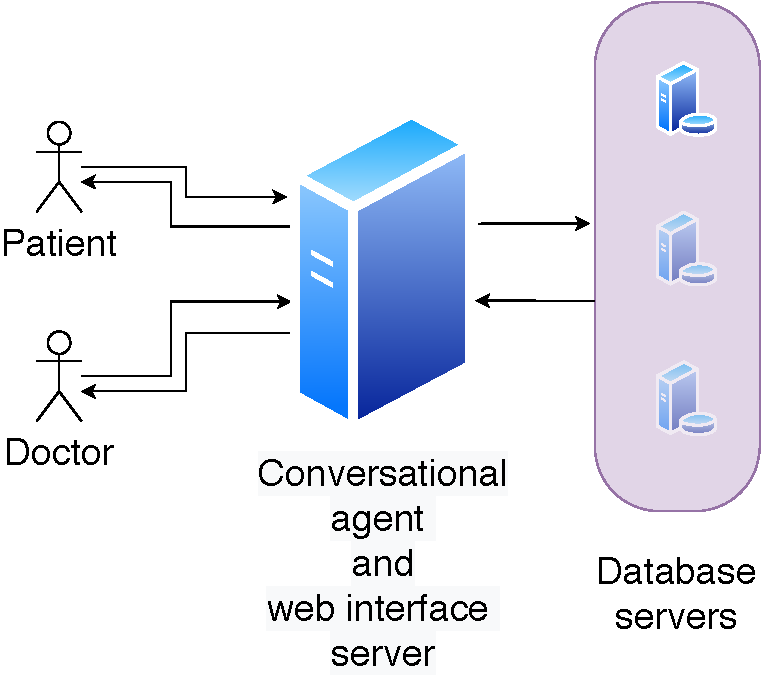
\includegraphics[width=0.7\textwidth]{non-scalable.pdf}
    \caption{Non-scalable environment architecture diagram. Created using \emph{diagrams.net} \protect\cite{drawio}.}
  \end{figure}
\end{frame}

\begin{frame}[fragile]{Production one-instance environment}
  \begin{figure}[H]
    \centering
    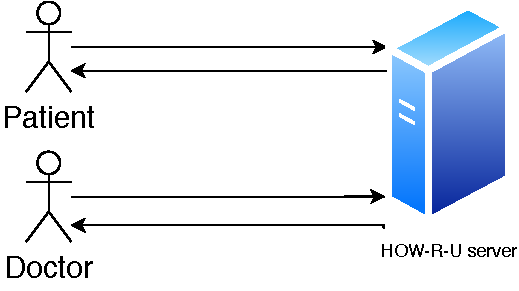
\includegraphics[width=0.7\textwidth]{one-instance.pdf}
    \caption{One-instance environment architecture diagram. Created using \emph{diagrams.net} \protect\cite{drawio}.}
  \end{figure}
\end{frame}


\section{Discussion and Conclussions}

\begin{frame}[fragile]{Discussion}
  \begin{figure}[H]
    \centering
    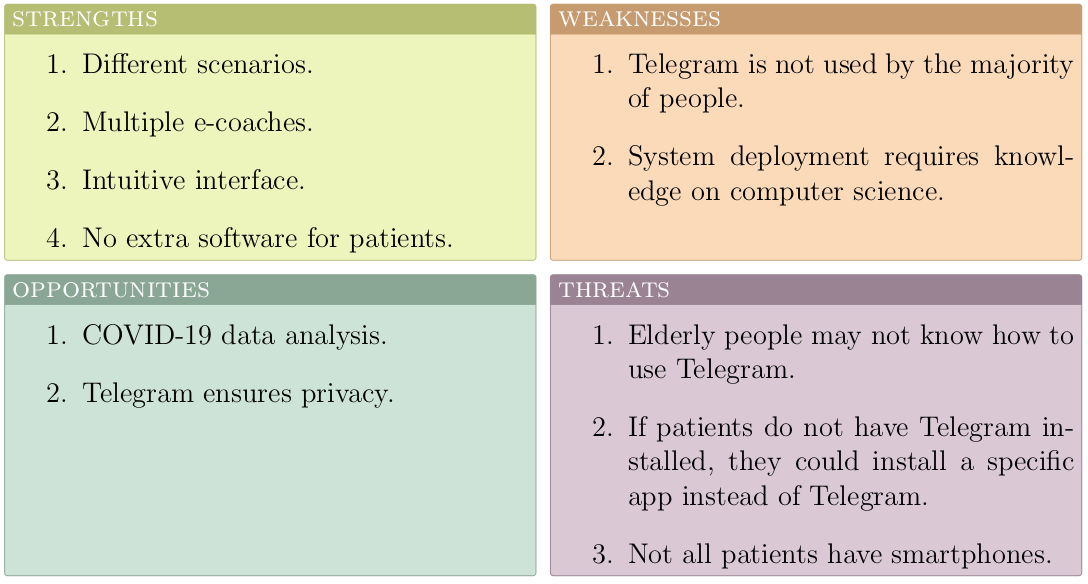
\includegraphics[width=\textwidth]{swot.png}
    \caption{HOW-R-U SWOT analysis. Based on \href{http://www.mostlycolor.ch/2015/07/swot-matrices-in-latex.html}{http://www.mostlycolor.ch/2015/07/swot-matrices-in-latex.html}.}
  \end{figure}
\end{frame}

\begin{frame}[fragile]{Conclussions}
  \begin{itemize}[<+->]
    \item \textbf{Main goal}: \emph{Conversational-agent-as-a-sensor} that asks questions defined by specialists to patients. \uncover<2-8>{\greentick}
    \item \textbf{Secondary goals}.
      \begin{itemize}[<+->]
        \item Graphical web interface for doctors. \uncover<4-8>{\greentick}
        \item Flexible and scalable architecture to add functionality to the system. \uncover<5-8>{\greentick}
        \item Architecture based on containers to host the different system modules. \uncover<6-8>{\greentick}
        \item Implement a system that covers the previous goals. \uncover<7-8>{\greentick}
        \item Test a beta version of the system to retrieve target audience’s feelings about it. \uncover<8>{\redcross}
      \end{itemize}
  \end{itemize}
\end{frame}

\section*{References}

\begin{frame}[allowframebreaks]{Bibliography}
\bibliographystyle{apacite}
\bibliography{refs}
\end{frame}

\begin{frame}{The end}
\begin{center}
  \Huge
  Time for questions
\end{center}
\end{frame}

\end{document}
